%\RequirePackage[l2tabu, orthodox]{nag}
\RequirePackage{currfile}
\documentclass[12pt]{beamer}
\graphicspath{{Imagenes/}{../Imagenes/}}
\usepackage[utf8]{inputenc}
\usepackage[spanish]{babel}
\usepackage{standalone}
\usepackage{color}
\usepackage[binary-units=true]{siunitx}
\usepackage{hyperref}
\hypersetup{
  colorlinks=true,
  linkcolor=blue,          % color of internal links (change box color with linkbordercolor)
  citecolor=green,        % color of links to bibliography
  filecolor=magenta,      % color of file links
  urlcolor=cyan,           % color of external links
  linkbordercolor={0 0 1}
}
\usepackage{xcolor, soul}
\usepackage{etoolbox}
\usepackage{amsmath}
\usepackage{amsthm}
\usepackage{physics}
\usepackage{multicol}
\usepackage{graphicx}
\usepackage{bookmark}
\usepackage{longtable}
\usepackage{graphicx}
\usepackage{tikz}
\usepackage[siunitx, RPvoltages]{circuitikz}
\usetikzlibrary{mindmap}
\usetikzlibrary{arrows, patterns, shapes, decorations.markings, decorations.pathmorphing}
\usetikzlibrary{matrix,positioning}
\tikzstyle{every picture}+=[remember picture,baseline]
\usepackage[autostyle,spanish=mexican]{csquotes}
\usepackage{pifont}
\usepackage[font=footnotesize,textfont=it]{caption}
\usepackage{tabulary}
\usepackage{booktabs}
\usepackage[outdir=./]{epstopdf}
%\usepackage{epstopdf}
\usepackage{media9}
\usepackage{multimedia}
\usepackage{bigints}
%\usepackage{enumitem}
\usepackage[os=win]{menukeys}
\usepackage{pifont}
\usepackage{pbox}
\usepackage{alltt}
\usepackage{verbatim}
\usepackage{colortbl}
\usepackage{tcolorbox}
\usepackage{fancyvrb}
\usepackage[sfdefault]{roboto}  %% Option 'sfdefault' only if the base font of the document is to be sans serif
%\usepackage[T1]{fontenc}
\setcounter{secnumdepth}{3}
\setcounter{tocdepth}{3}
\DeclareGraphicsExtensions{.pdf,.png,.jpg}
\renewcommand {\arraystretch}{1.5}
\definecolor{ao}{rgb}{0.0, 0.5, 0.0}
\definecolor{aquamarine}{rgb}{0.5, 1.0, 0.83}
\definecolor{kellygreen}{rgb}{0.3, 0.73, 0.09}
\definecolor{bisque}{rgb}{1.0, 0.89, 0.77}
\definecolor{amber}{rgb}{1.0, 0.75, 0.0}
\definecolor{armygreen}{rgb}{0.29, 0.33, 0.13}
\definecolor{alizarin}{rgb}{0.82, 0.1, 0.26}
\definecolor{cadetblue}{rgb}{0.37, 0.62, 0.63}
\newcommand*{\TitleParbox}[1]{\parbox[c]{6cm}{\raggedright #1}}%
\newcommand{\python}{\texttt{python}}
\newcommand{\textoazul}[1]{\textcolor{blue}{#1}}
\newcommand{\azulfuerte}[1]{\textcolor{blue}{\textbf{#1}}}
\newcommand{\funcionazul}[1]{\textcolor{blue}{\textbf{\texttt{#1}}}}
%\normalfont
\usepackage{ccfonts}% http://ctan.org/pkg/{ccfonts}
\usepackage[T1]{fontenc}% http://ctan.or/pkg/fontenc
\renewcommand{\rmdefault}{cmr}% cmr = Computer Modern Roman
\usefonttheme[onlymath]{serif}
\linespread{1.3}
\newcounter{saveenumi}
\newcommand{\seti}{\setcounter{saveenumi}{\value{enumi}}}
\newcommand{\conti}{\setcounter{enumi}{\value{saveenumi}}}
\newcommand{\tikzmark}[1]{\tikz[remember picture] \node[coordinate] (#1) {#1};}

\usepackage{scalerel}[2016-12-29]
\def\stretchint#1{\vcenter{\hbox{\stretchto[440]{\displaystyle\int}{#1}}}}
\def\scaleint#1{\vcenter{\hbox{\scaleto[3ex]{\displaystyle\int}{#1}}}}
\def\bs{\mkern-12mu}

\newtheorem{teo}{}[section]
\usepackage{blkarray}

%reduce el tamaño de letra de la etiqueta equations
\makeatletter
\def\maketag@@@#1{\hbox{\m@th\normalfont\small#1}}
\makeatother

%se usa para la x en itemize
\newcommand{\xmark}{\text{\ding{55}}}

%\AtBeginDocument{\setlength{\tymin}{1em}}


\definecolor{myblue}{rgb}{.8, .8, 1}

\usepackage{empheq}

\newlength\mytemplen
\newsavebox\mytempbox

\makeatletter
\newcommand\mybluebox{%
    \@ifnextchar[%]
       {\@mybluebox}%
       {\@mybluebox[0pt]}}

\def\@mybluebox[#1]{%
    \@ifnextchar[%]
       {\@@mybluebox[#1]}%
       {\@@mybluebox[#1][0pt]}}

\def\@@mybluebox[#1][#2]#3{
    \sbox\mytempbox{#3}%
    \mytemplen\ht\mytempbox
    \advance\mytemplen #1\relax
    \ht\mytempbox\mytemplen
    \mytemplen\dp\mytempbox
    \advance\mytemplen #2\relax
    \dp\mytempbox\mytemplen
    \colorbox{myblue}{\hspace{1em}\usebox{\mytempbox}\hspace{1em}}}

\makeatother



%Se usa la plantilla Warsaw modificada con spruce
\mode<presentation>
{
  \usetheme{Warsaw}
  \setbeamertemplate{headline}{}
  %\useoutertheme{infolines}
  \usecolortheme{spruce}
  \setbeamercovered{invisible}
  

\setbeamertemplate{section in toc}[sections numbered]
\setbeamertemplate{subsection in toc}[subsections numbered]
\setbeamertemplate{subsection in toc}{\leavevmode\leftskip=3.2em\rlap{\hskip-2em\inserttocsectionnumber.\inserttocsubsectionnumber}\inserttocsubsection\par}
\setbeamercolor{section in toc}{fg=blue}
\setbeamercolor{subsection in toc}{fg=blue}
\setbeamerfont{subsection in toc}{size=\small}



\setbeamertemplate{navigation symbols}{}
\setbeamertemplate{caption}[numbered]
% \setbeamercolor{frametitle}{fg=yellow,bg=blue!70!white}
%\setbeamercolor{section in head}{bg=green,fg=white}
%\setbeamercolor{subsection in head/foot}{bg=gray!30,fg=black}
%\setbeamercolor{author in head/foot}{fg=yellow}
%\setbeamercolor{date in head/foot}{fg=blue}

%\mode<presentation>
%{
%  \usetheme{Warsaw}
%  \setbeamertemplate{headline}{}
%  %\useoutertheme{infolines}
%  \useoutertheme{default}
%  \setbeamercovered{invisible}
%  % or whatever (possibly just delete it)
%}
}

\usepackage{courier}
\usepackage{listingsutf8}
\usepackage{listings}
\usepackage{xcolor}
\usepackage{textcomp}
\usepackage{color}
\definecolor{deepblue}{rgb}{0,0,0.5}
\definecolor{brown}{rgb}{0.59, 0.29, 0.0}
\definecolor{OliveGreen}{rgb}{0,0.25,0}
% \usepackage{minted}

\DeclareCaptionFont{white}{\color{white}}
\DeclareCaptionFormat{listing}{\colorbox{gray}{\parbox{0.98\textwidth}{#1#2#3}}}
\captionsetup[lstlisting]{format=listing,labelfont=white,textfont=white}
\renewcommand{\lstlistingname}{Código}


\definecolor{Code}{rgb}{0,0,0}
\definecolor{Keywords}{rgb}{255,0,0}
\definecolor{Strings}{rgb}{255,0,255}
\definecolor{Comments}{rgb}{0,0,255}
\definecolor{Numbers}{rgb}{255,128,0}

\makeatletter

\newif\iffirstchar\firstchartrue
\newif\ifstartedbyadigit
\newif\ifprecededbyequalsign

\newcommand\processletter
{%
  \ifnum\lst@mode=\lst@Pmode%
    \iffirstchar%
        \global\startedbyadigitfalse%
      \fi
      \global\firstcharfalse%
    \fi
}

\newcommand\processdigit
{%
  \ifnum\lst@mode=\lst@Pmode%
      \iffirstchar%
        \global\startedbyadigittrue%
      \fi
      \global\firstcharfalse%
  \fi
}

\lst@AddToHook{OutputOther}%
{%
  \lst@IfLastOtherOneOf{=}
    {\global\precededbyequalsigntrue}
    {}%
}

\lst@AddToHook{Output}%
{%
  \ifprecededbyequalsign%
      \ifstartedbyadigit%
        \def\lst@thestyle{\color{orange}}%
      \fi
    \fi
  \global\firstchartrue%
  \global\startedbyadigitfalse%
  \global\precededbyequalsignfalse%
}

\lstset{ 
language=Python,                % choose the language of the code
basicstyle=\footnotesize\ttfamily,       % the size of the fonts that are used for the code
numbers=left,                   % where to put the line-numbers
numberstyle=\scriptsize,      % the size of the fonts that are used for the line-numbers
stepnumber=1,                   % the step between two line-numbers. If it is 1 each line will be numbered
numbersep=5pt,                  % how far the line-numbers are from the code
backgroundcolor=\color{white},  % choose the background color. You must add \usepackage{color}
showspaces=false,               % show spaces adding particular underscores
showstringspaces=false,         % underline spaces within strings
showtabs=false,                 % show tabs within strings adding particular underscores
frame=single,   		% adds a frame around the code
tabsize=2,  		% sets default tabsize to 2 spaces
captionpos=t,   		% sets the caption-position to bottom
breaklines=true,    	% sets automatic line breaking
breakatwhitespace=false,    % sets if automatic breaks should only happen at whitespace
escapeinside={\#},  % if you want to add a comment within your code
stringstyle =\color{OliveGreen},
%otherkeywords={{as}},             % Add keywords here
keywordstyle = \color{blue},
commentstyle = \color{black},
identifierstyle = \color{black},
literate=%
         {á}{{\'a}}1
         {é}{{\'e}}1
         {í}{{\'i}}1
         {ó}{{\'o}}1
         {ú}{{\'u}}1
%
%keywordstyle=\ttb\color{deepblue}
%fancyvrb = true,
}

\lstdefinestyle{FormattedNumber}{%
    literate={0}{{\textcolor{red}{0}}}{1}%
             {1}{{\textcolor{red}{1}}}{1}%
             {2}{{\textcolor{red}{2}}}{1}%
             {3}{{\textcolor{red}{3}}}{1}%
             {4}{{\textcolor{red}{4}}}{1}%
             {5}{{\textcolor{red}{5}}}{1}%
             {6}{{\textcolor{red}{6}}}{1}%
             {7}{{\textcolor{red}{7}}}{1}%
             {8}{{\textcolor{red}{8}}}{1}%
             {9}{{\textcolor{red}{9}}}{1}%
             {.0}{{\textcolor{red}{.0}}}{2}% Following is to ensure that only periods
             {.1}{{\textcolor{red}{.1}}}{2}% followed by a digit are changed.
             {.2}{{\textcolor{red}{.2}}}{2}%
             {.3}{{\textcolor{red}{.3}}}{2}%
             {.4}{{\textcolor{red}{.4}}}{2}%
             {.5}{{\textcolor{red}{.5}}}{2}%
             {.6}{{\textcolor{red}{.6}}}{2}%
             {.7}{{\textcolor{red}{.7}}}{2}%
             {.8}{{\textcolor{red}{.8}}}{2}%
             {.9}{{\textcolor{red}{.9}}}{2}%
             {\ }{{ }}{1}% handle the space
         ,%
          %mathescape=true
          escapeinside={__}
          }



\makeatletter
\setbeamercolor{section in foot}{bg=gray!30, fg=black!90!orange}
\setbeamercolor{subsection in foot}{bg=blue!30!yellow, fg=red}
\setbeamertemplate{footline}
{
  \leavevmode%
  \hbox{%
  \begin{beamercolorbox}[wd=.333333\paperwidth,ht=2.25ex,dp=1ex,center]{section in foot}%
    \usebeamerfont{section in foot} \insertsection
  \end{beamercolorbox}}%
  \begin{beamercolorbox}[wd=.333333\paperwidth,ht=2.25ex,dp=1ex,center]{subsection in foot}%
    \usebeamerfont{subsection in foot}  \insertsubsection
  \end{beamercolorbox}%
  \begin{beamercolorbox}[wd=.333333\paperwidth,ht=2.25ex,dp=1ex,right]{date in head/foot}%
    \usebeamerfont{date in head/foot} \insertshortdate{} \hspace*{2em}
    \insertframenumber{} / \inserttotalframenumber \hspace*{2ex} 
  \end{beamercolorbox}}%
  \vskip0pt%
\makeatother
\title{Funciones de interpolación con \python}
%\subtitle{Funciones de interpolación con \texttt{python}}
\author{M. en C. Gustavo Contreras Mayén}
\begin{document}
\maketitle
\fontsize{14}{14}\selectfont
\spanishdecimal{.}
\section*{Contenido}
\frame{\tableofcontents[currentsection, hideallsubsections]}
\section{Funciones de interpolación con \texttt{python}.}
\frame{\tableofcontents[currentsection, hideothersubsections]}
\subsection{Paquete \texttt{scipy}}
\begin{frame}
\frametitle{Paquete para interpolación}
Encontramos en \python\ una serie de funciones que permiten realizar la interpolación de un conjunto de datos, estimando la mejor aproximación.
\\
\bigskip
No debemos de confiarnos en dar por hecho que con ello, el error obtenido por la aproximación es el menor.
\end{frame}
\begin{frame}
\frametitle{Paquete \texttt{scipy}}
El paquete que debemos de utilizar el \funcionazul{scipy}.
\\
\bigskip
Que a su vez contiene varias librerías de funciones para cómputo científico.
\end{frame}
\begin{frame}
\frametitle{Algunas librerías de \texttt{scipy}}
\begin{table}
\fontsize{12}{12}\selectfont
\centering
\begin{tabular}{l l}
Propósito & Librería \\ \hline
Funciones especiales & \texttt{scipy.special} \\ \hline
Integración &\texttt{scipy.integrate} \\ \hline
Optimización & \texttt{scipy.optimize} \\ \hline
\textcolor{red}{Interpolación} & \texttt{scipy.interpolate} \\ \hline
Transformadas de Fourier & \texttt{scipy.fft} \\ \hline
Procesamiento de señales & \texttt{scipy.signal} \\ \hline 
Álgebra lineal & \texttt{scipy.linalg} \\ \hline
\end{tabular}
\end{table}
\end{frame}
\subsection{La función \texttt{interp1d (x, y)}}
\begin{frame}[fragile]
\frametitle{La función \texttt{interp1d (x, y)}}
Dentro de \funcionazul{scipy.interpolate} contamos con la función \funcionazul{interp1d} que requiere de al menos dos argumentos: los valores de $x$ e $y$ que se utilizarán para la interpolación.
\\
\bigskip
\verb|interp1d(x, y, [kind='linear'])|
\\
\bigskip
Donde: \texttt{kind=} especifica el tipo de procedimiento de interpolación.
\end{frame}
\begin{frame}
\frametitle{Tipos de interpolación}
Las opciones disponibles son:
\setbeamercolor{item projected}{bg=red!70!black,fg=white}
\setbeamertemplate{enumerate items}[circle]
\begin{enumerate}[<+->]
\item \texttt{linear}: interpola a lo largo de una línea recta entre puntos de datos vecinos.
\item \texttt{nearest}: proyecta al punto de datos más cercano.
\item \texttt{zero}: proyecta al punto de datos anterior.
\item \texttt{slinear}: usa un \emph{spline} lineal.
\item \texttt{cuadratic}: usa un \emph{spline} cuadrático.
\item \texttt{cubic}: usa un \emph{spline} cúbico.
\end{enumerate}
\end{frame}
\begin{frame}
\frametitle{Sobre los splines}
Más adelante hablaremos sobre los \emph{splines}, que resultarán de gran ayuda no sólo para una interpolación, sino para tareas tan comunes como el trazo de líneas en programas de diseño por computadora.
\end{frame}
\begin{frame}[fragile]
\frametitle{Valor por defecto}
El valor predeterminado de \texttt{interp1d} es una \textcolor{blue}{interpolación lineal}.
\\
\bigskip
También se puede proporcionar un número entero, en cuyo caso la función utilizará un polinomio de ese orden para interpolar entre puntos.
\end{frame}
\begin{frame}[fragile]
\frametitle{Polinomio de orden $n$}
Por ejemplo:
\begin{verbatim}
F = interp1d (x, y, kind = 10)
\end{verbatim}
Utilizará un polinomio de orden 10 para interpolar entre los puntos $x$ e $y$.
\end{frame}
\begin{frame}
\frametitle{Comparando los tipos de interpolación}
Veamos con un ejemplo sencillo las diferencias entre los tipos de interpolación lineal y cúbica que se tienen para la función \funcionazul{interp1d}:
\end{frame}
\begin{frame}[fragile]
\frametitle{Ejemplo}
Con el siguiente código generamos un conjunto de 20 datos distribuidos entre $0$ y $10 * \pi$, para luego presentarlos en una gráfica:
\end{frame}
\begin{frame}[fragile]
\frametitle{Ejemplo}
\begin{lstlisting}[caption=Generando los puntos, style= FormattedNumber, basicstyle=\linespread{0.9}\ttfamily\small, columns=fullflexible]
import numpy as np
from scipy.interpolate import interp_1_d
import matplotlib.pyplot as plt

x = np.linspace(0, 10 * np.pi, 20)
y = np.cos(x)

# graficamos los puntos

plt.plot(x, y, 'bo', label='Datos')
plt.legend(loc=1)
plt.show()
\end{lstlisting}
\end{frame}
\begin{frame}
\frametitle{Mostrando la gráfica}
\begin{figure}
%\centering
\hspace*{-0.2cm}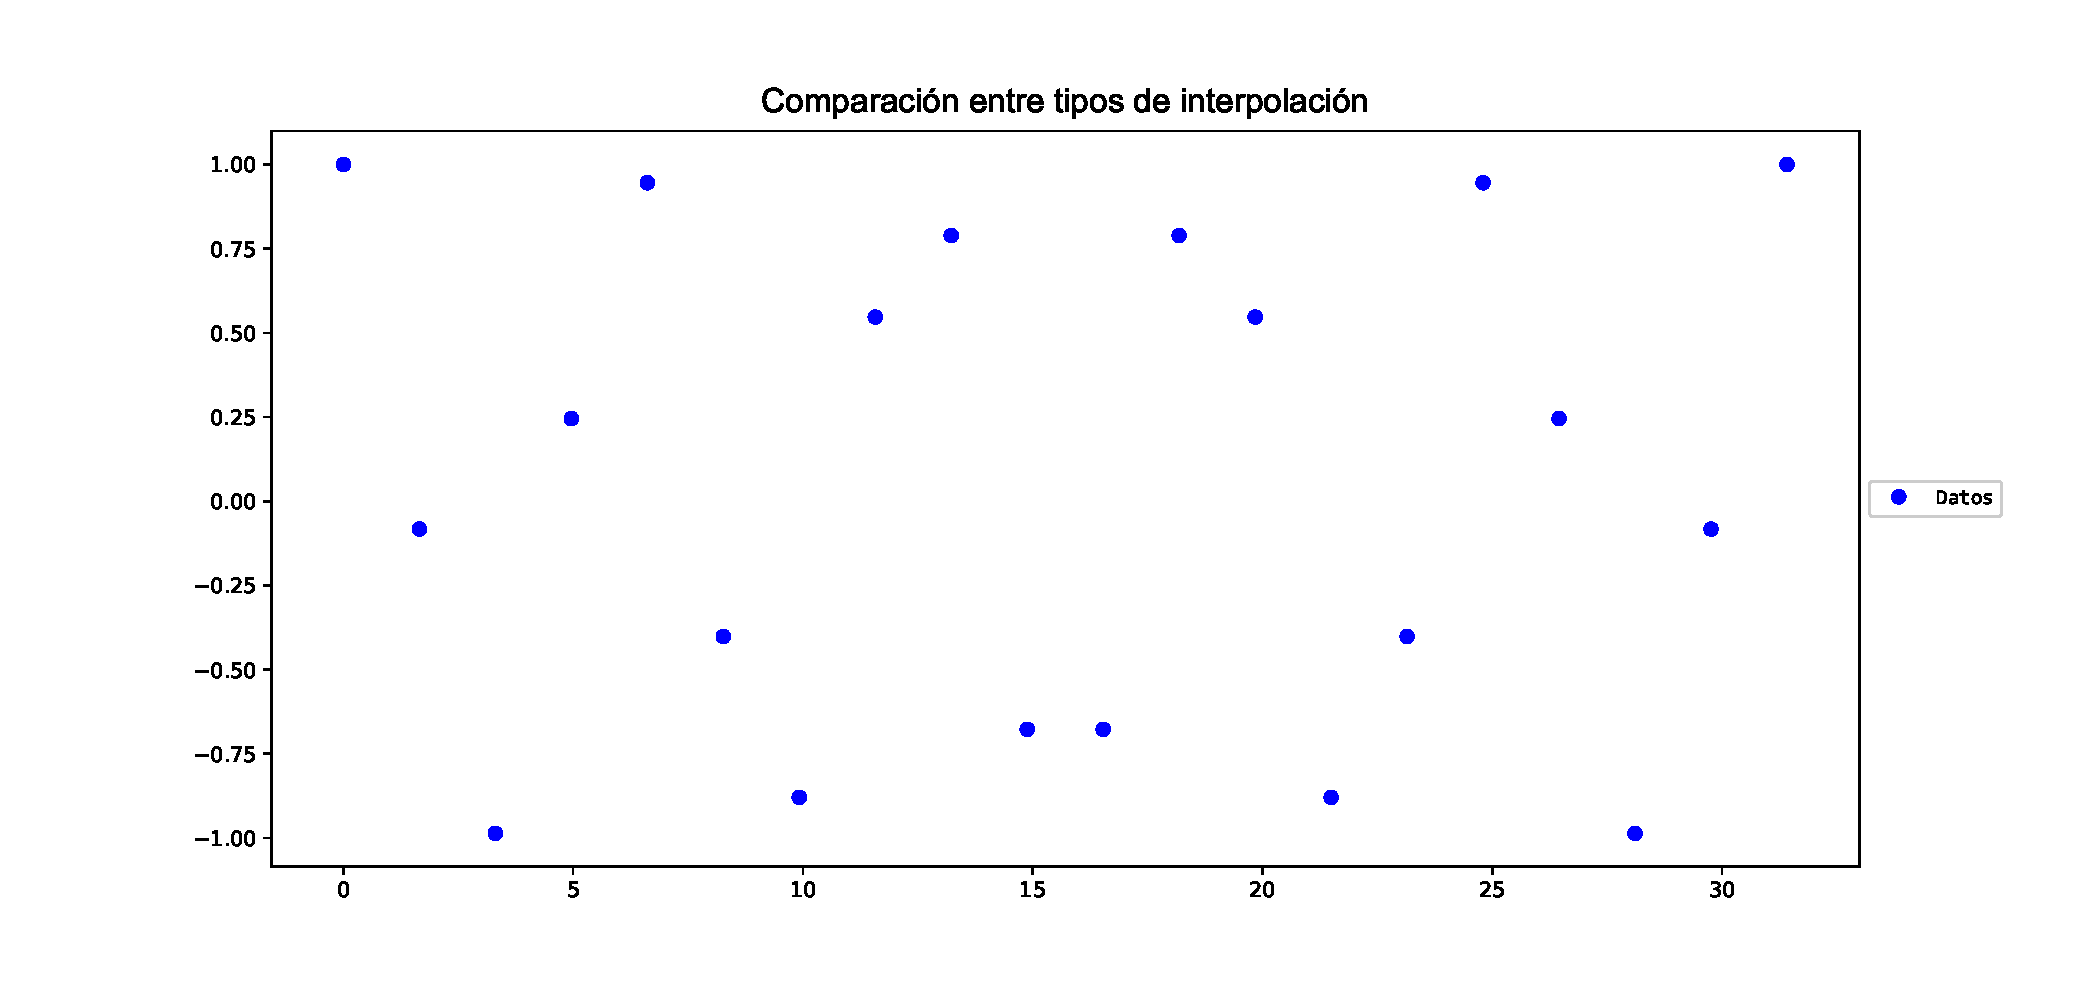
\includegraphics[scale=0.3]{interpolacion_01.eps}
\end{figure}
\end{frame}
\begin{frame}
\frametitle{Interpolación lineal y cuadrática}
Ocuparemos la interpolación lineal y cúbica de la función \funcionazul{inter1d}, para comparar gráficamente el resultado, por lo que se utilizará en dos ocasiones la función \funcionazul{interp1d}.
\\
\bigskip
La parte correspondiente a la graficación se incluye en el código anterior, para no repetir las funciones \texttt{legend(loc=1)} y \texttt{show()}.
\end{frame}
\begin{frame}[allowframebreaks, fragile]
\frametitle{Se interpolan los datos}
\begin{lstlisting}[caption=Definiendo el tipo de interpolación, style= FormattedNumber, basicstyle=\linespread{0.9}\ttfamily\small, columns=fullflexible]

fl = interp_1_d(x, y, kind='linear')

fq = interp_1_d(x, y, kind='quadratic')

# x.min and x.max se usan para asegurar que no
# nos salimos del intervalo de interpolacion

xint = np.linspace(x.min(), x.max(), 1000)

yintl = fl(xint)

yintq = fq(xint)

#para graficar

plt.plot(xint, yintl, label='Lineal')
plt.plot(xint, yintq, label='Cubica')
\end{lstlisting}
\end{frame}
\begin{frame}
\frametitle{Interpolación lineal}
\begin{figure}
%\centering
\hspace*{-0.2cm}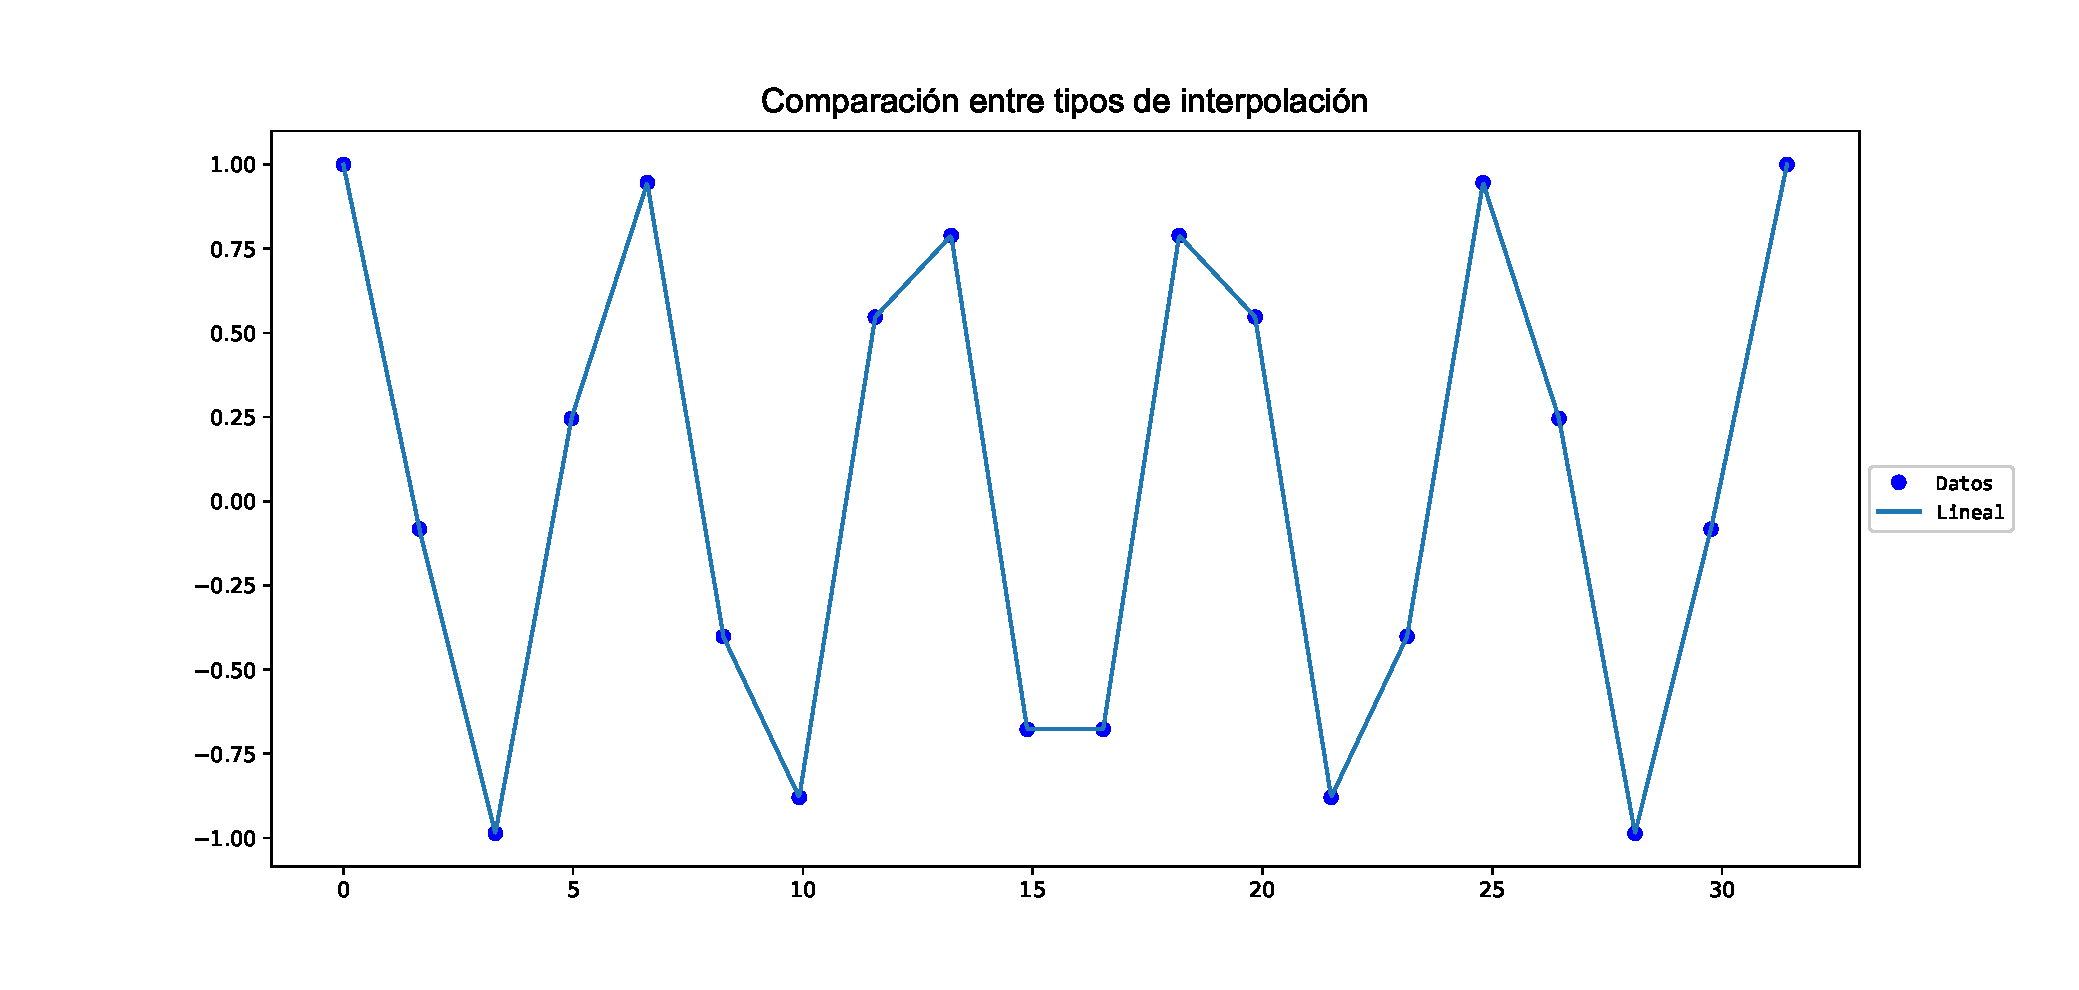
\includegraphics[scale=0.35]{interpolacion_02.eps}
\end{figure}
\end{frame}
\begin{frame}
\frametitle{Interpolación cúbica}
\begin{figure}
%\centering
\hspace*{-0.2cm}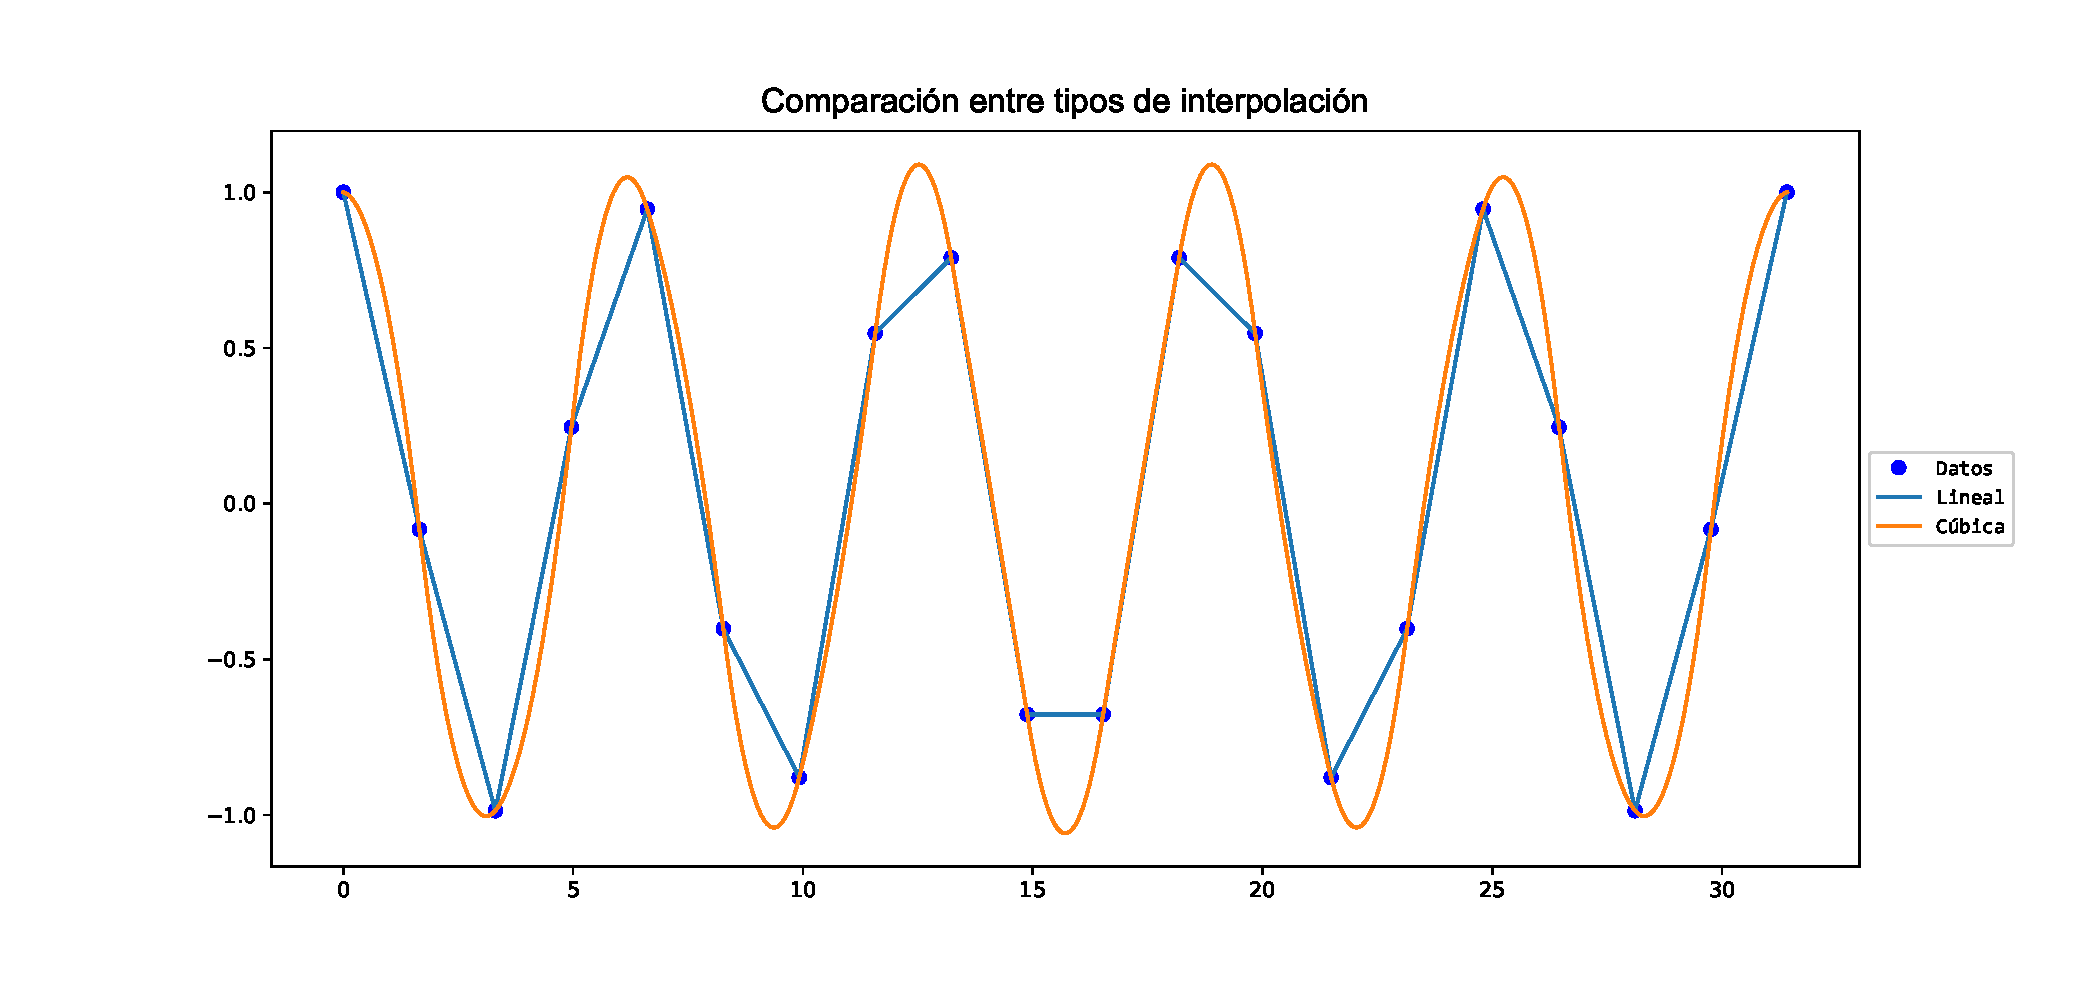
\includegraphics[scale=0.35]{interpolacion_03.eps}
\end{figure}
\end{frame}
\begin{frame}
\frametitle{Veamos otro ejemplo}
Utilizaremos la función \funcionazul{sinc(x)} que está contenida dentro del paquete \funcionazul{numpy}.
\\
\bigskip
\pause
La función \funcionazul{sinc (x)}, también llamada \enquote{función de muestreo}, es una función que se encuentra comúnmente de las teorías de procesamiento de señales y de las transformadas de Fourier.
\end{frame}
\begin{frame}
\frametitle{Función seno cardinal}
El nombre completo de la función es \enquote{seno cardinal}, pero es comúnmente referido por su abreviatura: \enquote{sinc}.
\\
\bigskip
Se define como
\begin{align*}
sinc(x) = \begin{cases}
1 & \mbox{para } x = 0 \\[0.5em]
\dfrac{\sin x}{x} & \mbox{para cualquier otro valor} \end{cases}
\end{align*}
\end{frame}
\begin{frame}
\frametitle{Otra función de \texttt{numpy}}
Para generar un conjunto de valores aleatorios, ocuparemos del paquete \funcionazul{numpy}, la librería \funcionazul{random} y de ésta, la función \funcionazul{random}.
\\
\bigskip
\pause
Que nos va a devolver un conjunto de valores de punto flotante en el intervalo $[0, 1]$.
\end{frame}
\begin{frame}[fragile]
\frametitle{la función \texttt{random}}
La sintaxis para la función \funcionazul{random} es la siguiente:
\\
\bigskip
\verb|numpy.random.random(valor)|
\\
\bigskip
donde \texttt{valor} es el tamaño de la muestra de datos aleatorios, en caso de que no se indique, se devuelve un sólo valor.
\end{frame}
\begin{frame}
\frametitle{Los datos iniciales}
La idea en este ejercicio es \enquote{contaminar} (modificar) la función \funcionazul{sinc(x)} y estudiar la interpolación lineal y cúbica con \python.
\\
\bigskip
Si sumamos los datos aleatorios a la función \funcionazul{sinc(x)}, tendremos una gráfica muy parecida a la esperada.
\end{frame}
\begin{frame}
\frametitle{Dos interpolaciones}
El conjunto de datos $x2$ nos servirá para interpolar con la función \funcionazul{interp1d}.
\\
\bigskip
Los arreglos $y$ y $y2$ almacenan los datos de las interpolaciones lineal y cúbica, respectivamente.
\end{frame}
\begin{frame}[fragile]
\frametitle{Código para resolver el ejercicio}
\begin{lstlisting}[caption=Código para el análisis, style= FormattedNumber, basicstyle=\linespread{0.9}\ttfamily\small, columns=fullflexible]
import numpy as np
from scipy.interpolate import interp_1_d

x = np.linspace(-18, 18, 36)
ruido = 0.1 * np.random.random(len(x))
senal = np.sinc(x) + ruido

x_2_ = np.linspace(-18, 18, 180)

interlineal = interp_1_d(x, senal)
y = interlineal(x_2_)

intercubica = interp_1_d(x, senal, kind="cubic")
y_2_ = intercubica(x_2_)
\end{lstlisting}
\end{frame}
\begin{frame}
\frametitle{Agregar rutina de graficación}
Deberás de incluir una rutina de graficación para mostrar tres gráficas:
\begin{itemize}
\item La función \funcionazul{sinc(x)}
\item La interpolación lineal.
\item La interpolación cúbica.
\end{itemize}
\end{frame}
\begin{frame}
\frametitle{Interpolación con la señal de muestreo}
\begin{figure}
%\centering
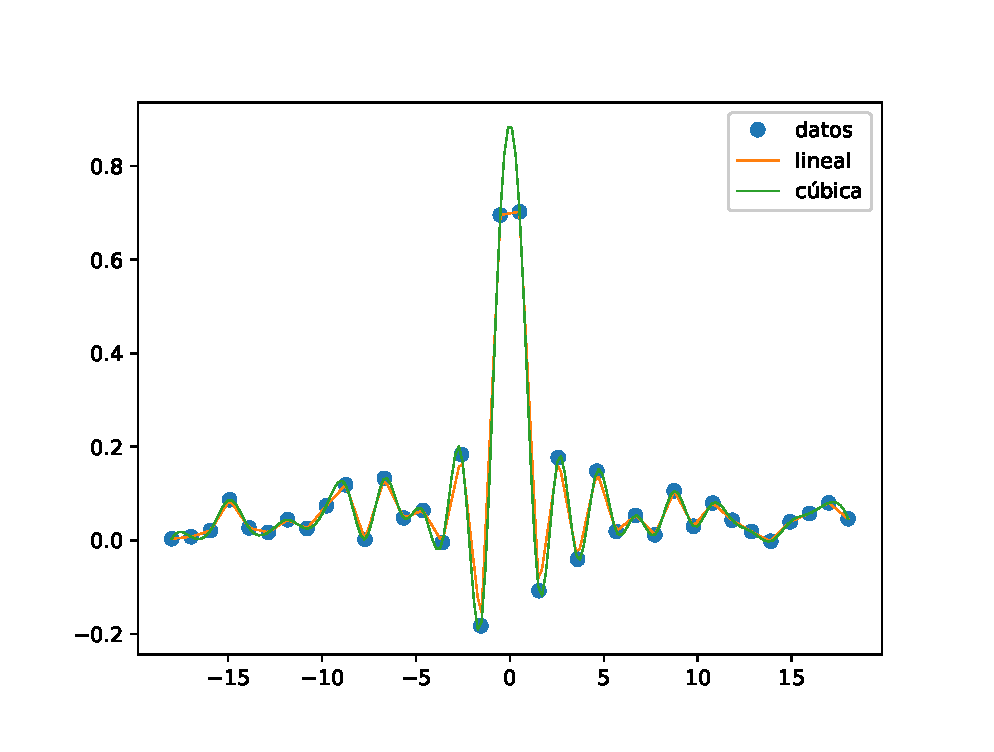
\includegraphics[scale=0.65]{interpolacion_04.eps}
\end{figure}
\end{frame}
\begin{frame}
\frametitle{Más sobre la interpolación}
Es posible reconocer algunas características generales de la interpolación obtenida en las gráficas:
\setbeamercolor{item projected}{bg=red!70!black,fg=white}
\setbeamertemplate{enumerate items}[circle]
\begin{enumerate}[<+->]
\item Las funciones de interpolación son continuas.
\item Las funciones de interpolación pasan siempre por los puntos de datos.
\item Una función cúbica puede dar un ajuste más malo que la interpolación lineal.
\seti
\end{enumerate}
\end{frame}
\begin{frame}
\frametitle{Más sobre la interpolación}
\setbeamercolor{item projected}{bg=red!70!black,fg=white}
\setbeamertemplate{enumerate items}[circle]
\begin{enumerate}[<+->]
\conti
\item Aumentar el orden del polinomio no siempre conduce a un mejor ajuste.
\item Las funciones de interpolación pueden oscilar drásticamente entre los puntos de datos.
\item El ajuste empeora hacia los extremos del conjunto de datos.
\end{enumerate}
\end{frame}
\begin{frame}
\frametitle{Entonces ¿qué hacemos?}
El \emph{spline cúbico} es el caballo de batalla en este terreno. 
\\
\bigskip
Como se puede ver en la siguiente figura, proporciona una curva suave que parece ajustarse bien a los datos.
\end{frame}
\begin{frame}
\frametitle{Entonces ¿qué hacemos?}
Interpolación son spline cúbico:
\begin{figure}
\centering
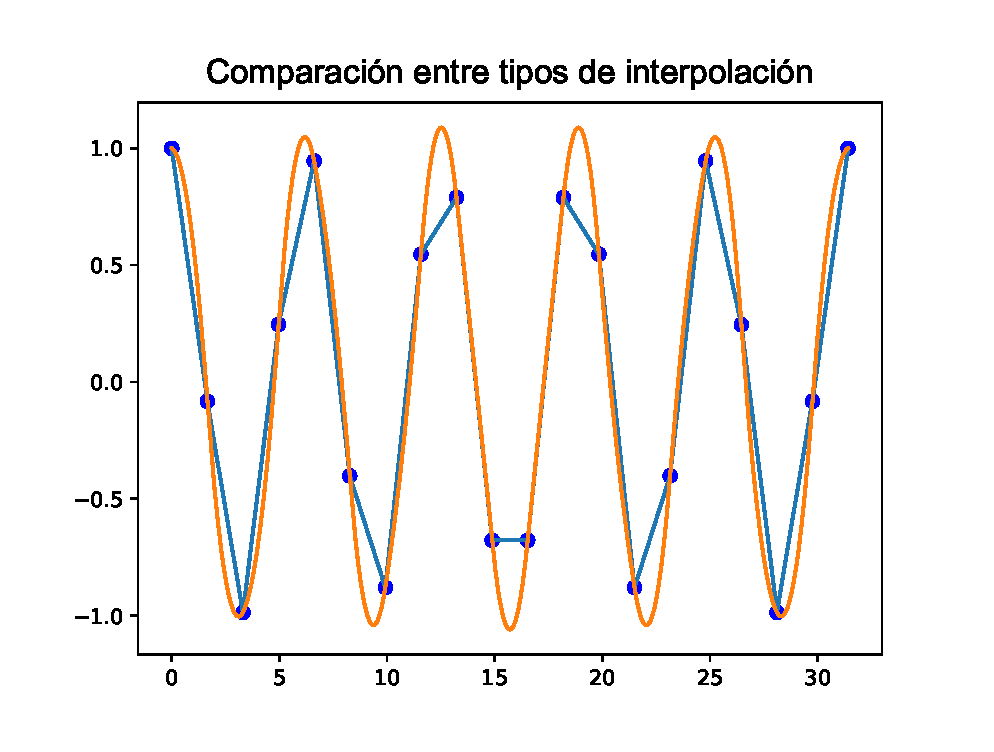
\includegraphics[scale=0.5]{interpolacion_03b.eps}
\end{figure}
\end{frame}
\begin{frame}
\frametitle{Ventaja del spline cúbico}
La suavidad se extiende más allá de lo que se ve en la gráfica: un \emph{spline cúbico} tiene derivadas primera y segunda continuas.
\end{frame}
\begin{frame}
\frametitle{Uso de la ventaja del spline cúbico}
Esta es una propiedad útil en la física, donde las derivadas primera y segunda son bastante comunes en los análisis teóricos (leyes de Newton, ecuaciones de Maxwell, ecuación de Schröedinger, etc.)
\\
\medskip
\pause
\textcolor{blue}{Una interpolación de spline cúbico es una buena opción en la mayoría de los casos}.
\end{frame}
\begin{frame}
\frametitle{Cuidado con la interpolación}
Precaución: la interpolación y la extrapolación no es lo mismo.
\\
\bigskip
Una buena función de interpolación puede ser una aproximación muy mala fuera del conjunto de puntos de datos utilizados. 
\end{frame}
\begin{frame}
\frametitle{Cuidado con la interpolación}
Por esta razón, las funciones generadas por \funcionazul{interp1d (x, y)} ni siquiera devolverán un número cuando proporcione un valor de la variable independiente fuera del rango del conjunto de datos: se obtiene un \texttt{ValueError} en su lugar.
\end{frame}
\section{Fenómeno de Runge}
\begin{frame}
\frametitle{Fenónemo de Runge}
Hasta el momento hemos revisado un par de estrategias para calcular un polinomio que pase por un conjunto de datos $(x_{i}, y_{i})$, pero hay que considerar un efecto importante al respecto: no siempre el mejor polinomio será aquel el de mayor grado $n$.
\end{frame}
\begin{frame}
\frametitle{Fenónemo de Runge}
Veamos el siguiente ejemplo: sea la función:
\begin{align*}
f(x) = \dfrac{1}{1 + 25 x^{2}}
\end{align*}
\end{frame}
\begin{frame}
\frametitle{Gráfica de la función $f(x)$}
\begin{figure}
	\centering
	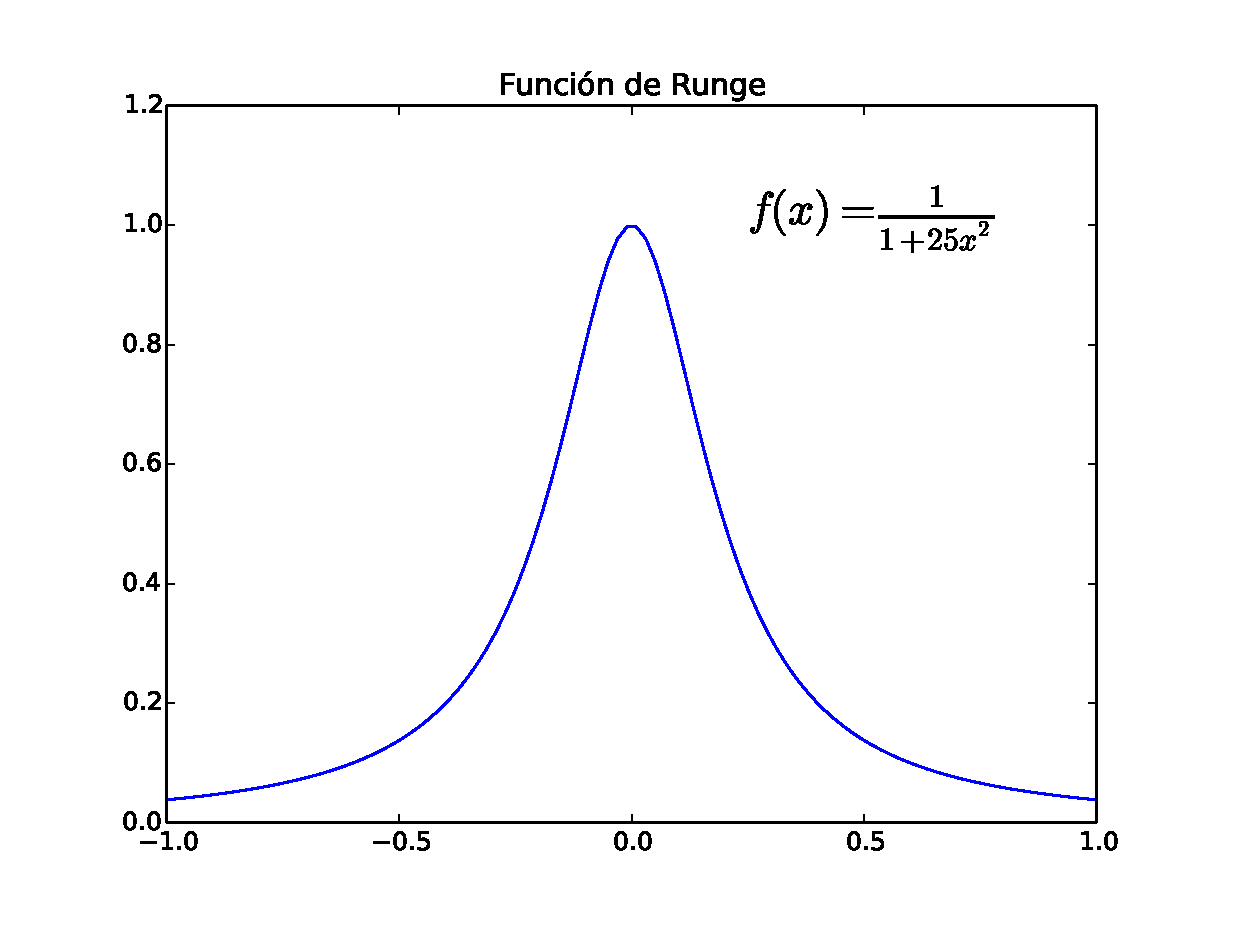
\includegraphics[scale=0.5]{Imagenes/Funcion_Runge_01.eps} 
\end{figure}
\end{frame}
\begin{frame}
\frametitle{Elección de puntos}
Como en los ejercicios anteriores, elegimos un conjunto de puntos que nos servirán para interpolar, en este caso, mostraremos las gráficas resultantes (sería buena idea de que hicieran todo el ejercicio por su cuenta)
\end{frame}
\begin{frame}
\frametitle{Elección de puntos para interpolar}
\begin{figure}
	\centering
	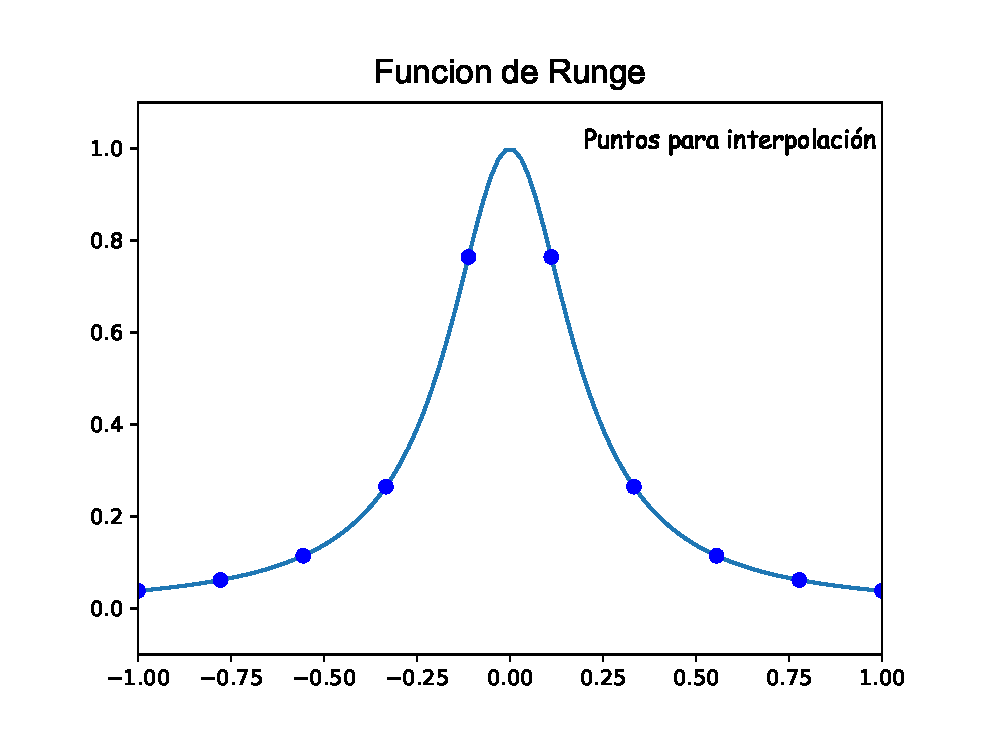
\includegraphics[scale=0.5]{Imagenes/Funcion_Runge_2017_01.eps} 
\end{figure}
\end{frame}
\begin{frame}
\frametitle{Interpolación con Lagrange}
Interpolando los puntos con el método de Lagrange.
\begin{figure}
	\centering
	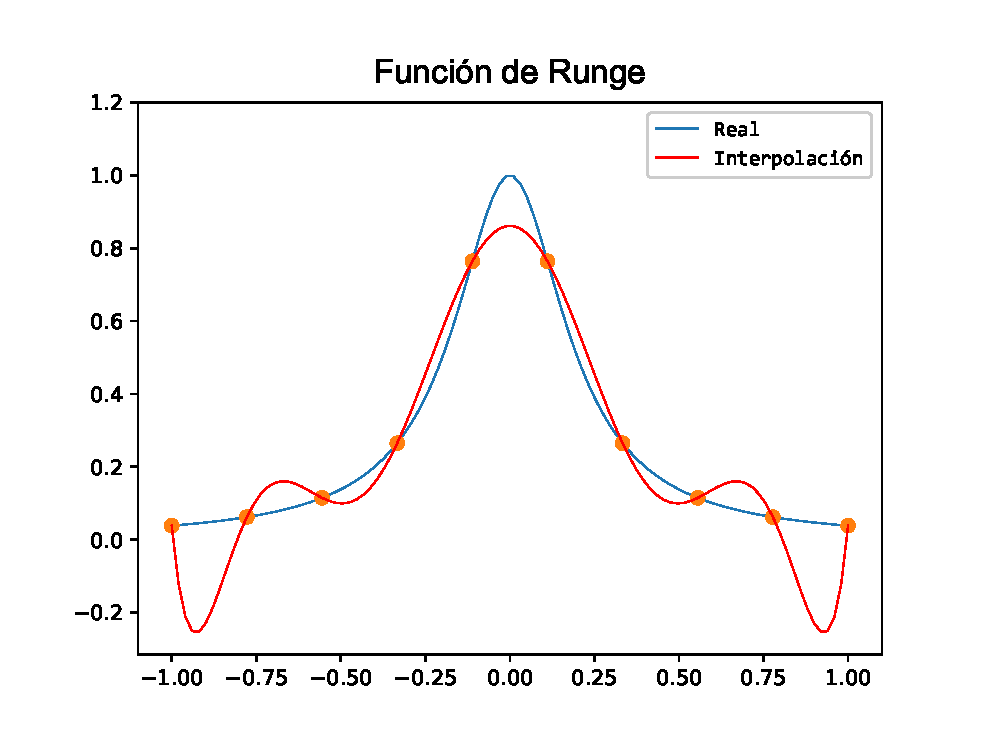
\includegraphics[scale=0.5]{Imagenes/Funcion_Runge_2017_02.eps} 
\end{figure}
\end{frame}
\begin{frame}
\frametitle{¿Qué hacemos al respecto?}
Como hemos visto en la gráfica anterior, la función que resulta del proceso de interpolación \enquote{oscila} a través de los puntos que deseamos interpolar.
\\
\bigskip
\pause
Si aumentamos el grado del polinomio, los resultados serán aún más indeseables.
\end{frame}
\begin{frame}
\frametitle{¿Qué hacemos al respecto?}
La pregunta obligada es: ¿qué podemos hacer para mejorar la interpolación?
\\
\bigskip
\pause
La respuesta a la pregunta es: usemos \emph{splines}.
\end{frame}
\subsection{Uso de splines}
\begin{frame}
\frametitle{¿Qué es un spline?}
En términos nada riguroso, se puede decir que un \emph{spline} es una función definida por una familia de polinomios \emph{sociables}, donde el término sociable se usa para indicar que los polinomios que constituyen una función spline, están estrechamente vinculados.
\end{frame}
\begin{frame}
\frametitle{¿Qué es un spline?}
El nombre de \emph{spline}, viene del inglés ya que es un instrumento que utilizaban los ingenieros navales para dibujar curvas suaves, forzadas a pasar por un conjunto de puntos prefijados.
\end{frame}
\begin{frame}
\frametitle{Un spline}
\begin{figure}
	\centering
	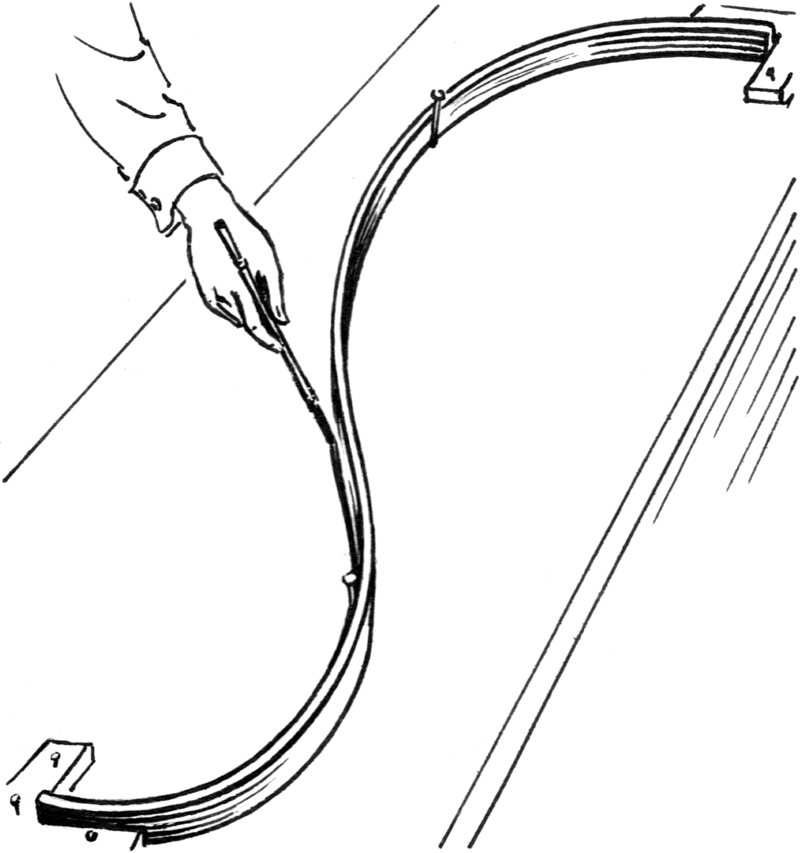
\includegraphics{Imagenes/spline_01.png}
	\caption{Uso de un spline para trazar curvas.}
	\label{fig:figura_spline_01}
\end{figure}
\end{frame}
\begin{frame}
\frametitle{Un spline moderno}
\begin{figure}
	\centering
	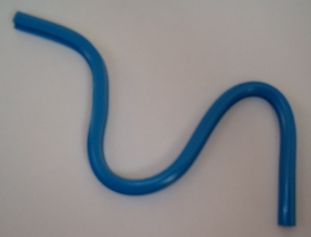
\includegraphics[scale=0.5]{Imagenes/spline_02.jpg}
	\caption{Un spline moderno para trazo de curvas.}
	\label{fig:figura_spline_02}
\end{figure}
	\end{frame}
\begin{frame}
\frametitle{Las tres B's de los splines}
El uso de las funciones splines tiene mucha aceptación y popularidad se deben a tres razones básicas:
\setbeamercolor{item projected}{bg=red!70!black,fg=white}
\setbeamertemplate{enumerate items}[circle]
\begin{enumerate}[<+->]
\item \textbf{Buenos:} Se  pueden usar en la solución de una gran variedad de problemas.
\item \textbf{Bonitos:} La teoría matemática en que se basan es muy simple y a la vez elegante.
\item \textbf{Baratos:} Ya que su cálculo es muy sencillo y económico.
\end{enumerate}
\end{frame}
\begin{frame}
\frametitle{Teoría de los splines}
No está de más que revises la teoría al respecto, en la mayoría de los libros de análisis numérico, podrás encontrar la construcción matemática y formal de los splines.
\end{frame}
\begin{frame}
\frametitle{Funciones de \python{} para los splines}
Necesitaremos ocupar nuevamente el paquete \funcionazul{scipy} y la librería \funcionazul{interpolate}, de donde utilizaremos dos funciones para los splines:
\setbeamercolor{item projected}{bg=blue!70!black,fg=yellow}
\setbeamertemplate{enumerate items}[circle]
\begin{enumerate}[<+->]
\item La función \funcionazul{splrep}.
\item La función \funcionazul{splev}.
\end{enumerate}
\end{frame}
\begin{frame}[fragile]
\frametitle{Funciones de \python{} para los splines}
De donde:
\setbeamercolor{item projected}{bg=blue!70!black,fg=yellow}
\setbeamertemplate{enumerate items}[circle]
\begin{enumerate}[<+->]
\item \textbf{splrep}: Calcula el spline básico (B-spline) para una curva 1-D.
\\
\medskip
\verb|splrep(x, y)|
\\
\bigskip
Dados un conjunto de puntos $(x[i], \, y[i])$ determina una aproximación con un spline suave de grado $k$ en el intervalo $xb \leq x \leq xe$.
\seti
\end{enumerate}
\end{frame}
\begin{frame}[fragile]
\frametitle{Lo que devuelve \texttt{splrep}}
Esta función devuelve lo siguiente:
\\
\bigskip
\verb|tck|
\\
\bigskip
Una tupla \texttt{(t, c, k)} que contiene:
\begin{itemize}
\item Un arreglo $t$ con los nodos.
\item Un arreglo $c$ con los coeficientes del B-spline.
\item Un valor $k$ que determina el grado del spline.
\end{itemize}
\end{frame}
\begin{frame}[fragile]
\frametitle{Funciones de \python{} para los splines}
\setbeamercolor{item projected}{bg=blue!70!black,fg=yellow}
\setbeamertemplate{enumerate items}[circle]
\begin{enumerate}[<+->]
\conti
\item \textbf{splev}: Evalúa un B-spline o sus derivadas. 
\\
\bigskip
\verb|splev(x, tck)|
\\
\bigskip
Dados los nodos y coeficientes de un B-spline que devuelve \funcionazul{splrep}, entonces calcula el valor del polinomio suave y sus derivadas.
\end{enumerate}
\end{frame}
\begin{frame}
\frametitle{Lo que devuelve \texttt{splev}}
La función \funcionazul{splev} devuelve un arreglo de valores que representan el spline evaluado en los puntos $x$.
\end{frame}
\begin{frame}
\frametitle{Implementando el código}
Ocuparemos la función inicial \emph{Runge} en el intervalo $[-1, \, 1]$
\\
\bigskip
\pause
Haremos dos ajustes con splines, uno para $n = 8$ puntos y otro para $n = 16$ puntos.
\end{frame}
\begin{frame}
\frametitle{Implementando el código}
La función \funcionazul{trazador(n)} va a generar el conjunto de datos $x_{i}, y_{i}$ que servirán como parámetros para la función \funcionazul{splrep}, recuperamos la tupla \funcionazul{tck} en cada caso.
\end{frame}
\begin{frame}[allowframebreaks, fragile]
\frametitle{Código para el ejercicio}
\begin{lstlisting}[caption=Código para el ejercicio, style= FormattedNumber, basicstyle=\linespread{0.9}\ttfamily\small, columns=fullflexible]
from numpy import linspace
from scipy.interpolate import splrep, splev
import matplotlib.pyplot as plt

x = linspace(-1, 1, 100)
y = 1./(1 + 25 * x**2)

def trazadorcub(n):
    xi = linspace(-1, 1, n)
    yi = 1./(1 + 25 * xi**2)
    tck = splrep(xi, yi)
    return tck

tck = trazadorcub(8)
ys_8_ = splev(x, tck)

tck = trazadorcub(12)
ys_12_ = splev(x, tck)

plt.plot(x, y, label='f(x)')
plt.plot(x, ys_8_,'+g-', label='n=8')
plt.plot(x, ys_12_,'+r-',label ='n=12')
plt.legend(loc='best')
plt.title('Interpolacion con splines cubicos')
plt.ylim(-0.2, 1.2)
plt.axhline(y=0, ls='dashed', lw=0.7, color='k')
plt.show()
\end{lstlisting}
\end{frame}
\begin{frame}
\frametitle{Resultados gráficos}
\begin{figure}
	\centering
	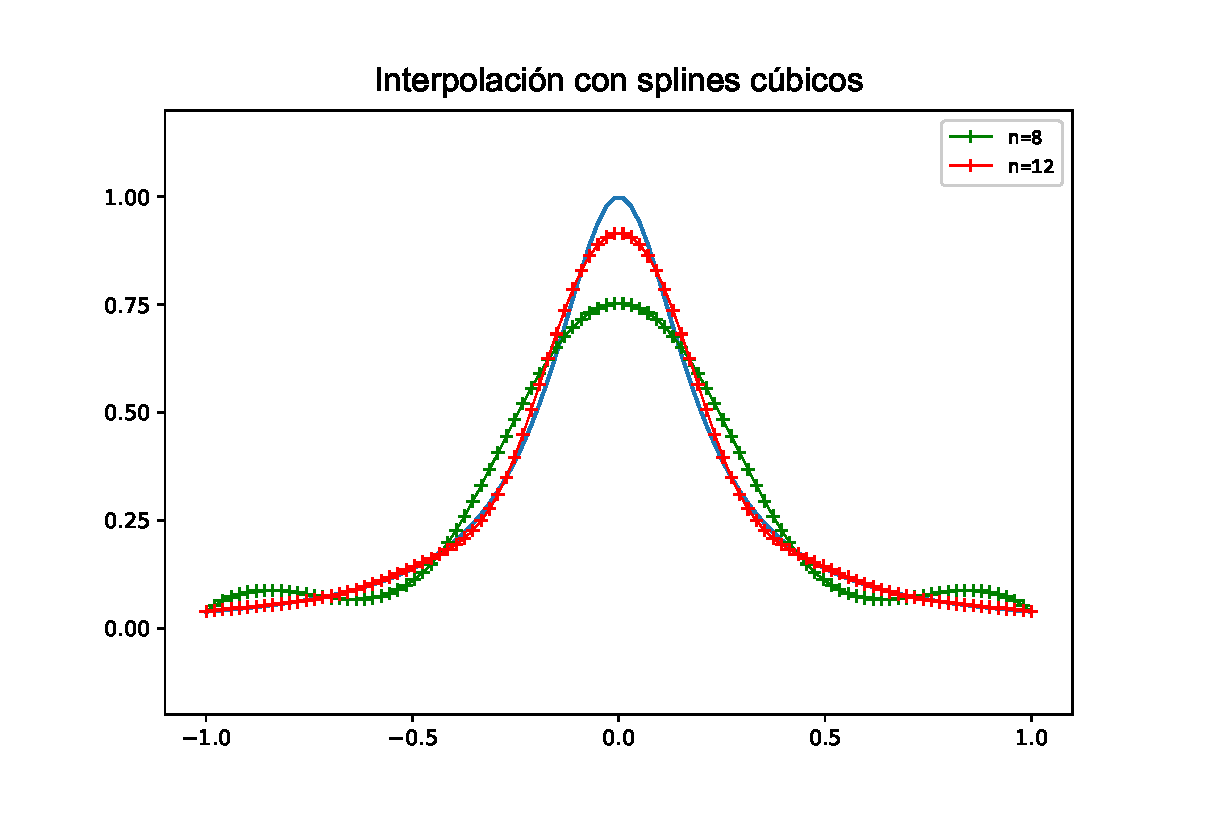
\includegraphics[scale=0.5]{Imagenes/Funcion_Runge_2017_03.eps} 
\end{figure}
\end{frame}
\begin{frame}
\frametitle{Conclusiones}
El uso de splines responde la pregunta que nos planteamos: garantizamos un mejor ajuste a la interpolación de un conjunto de datos.
\end{frame}
\begin{frame}
\frametitle{Uso de los splines}	
Los splines se han vuelto una herramienta cotidiana dentro de los programas de diseño gráfico.
\\
\bigskip
Una curva suave que aproxime un par de puntos o varios puntos, es lo que obtenemos cuando usamos los splines.
\end{frame}
\begin{frame}
\frametitle{Uso de los splines}
\begin{figure}[h!]
	\centering
	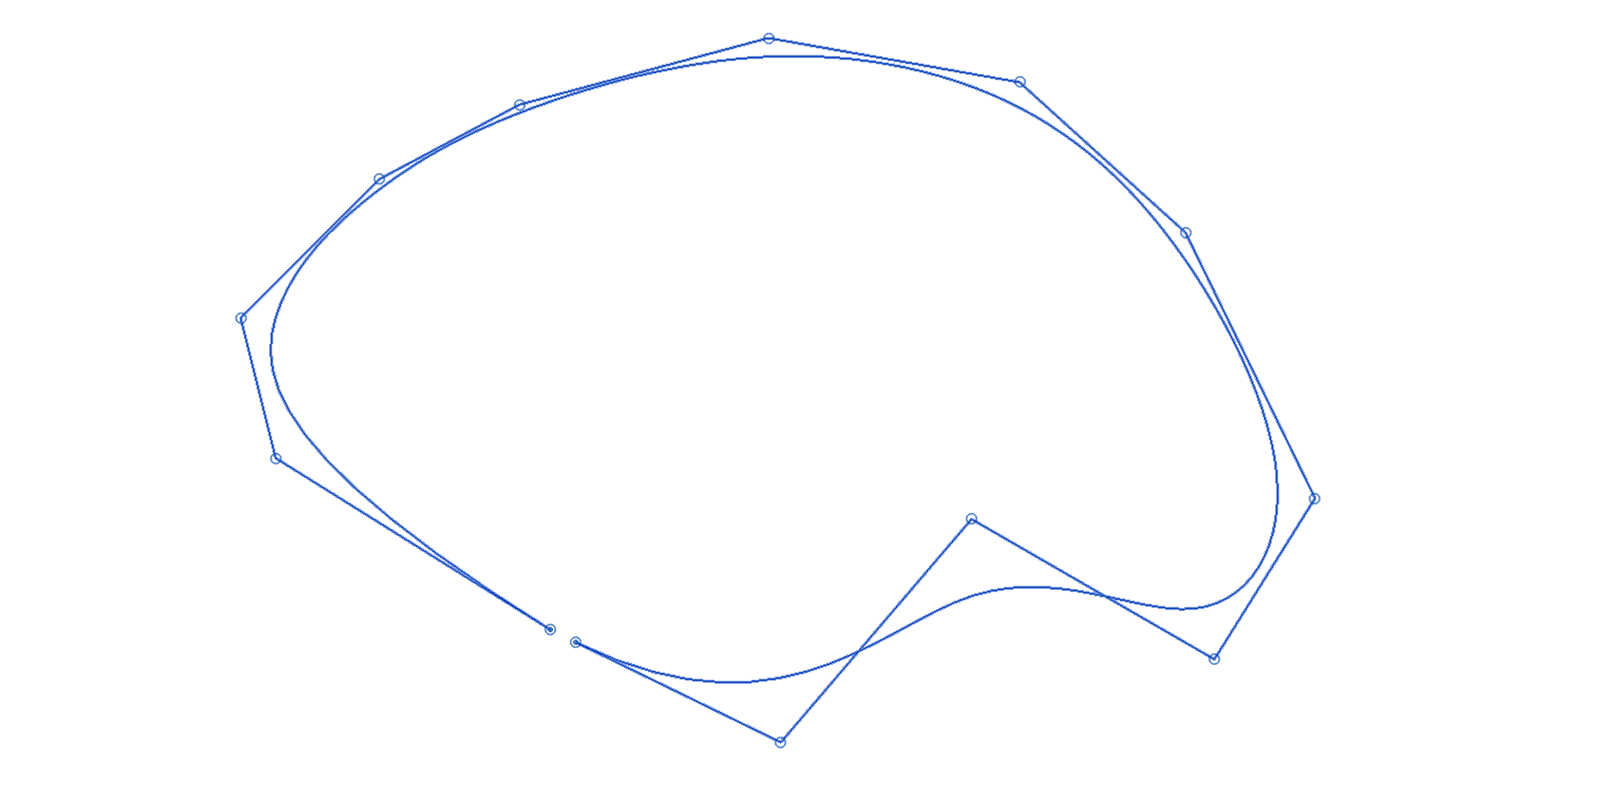
\includegraphics[scale=0.1]{Imagenes/spline_03.png}
	\caption{Trazo de una curva en un programa de diseño.}
	\label{fig:figura_spline_03}
\end{figure}
\end{frame}
\begin{frame}
\frametitle{Uso de los splines}
\begin{figure}[h!]
	\centering
	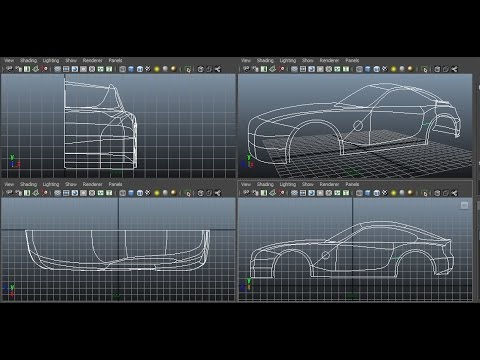
\includegraphics[scale=0.5]{Imagenes/spline_04.png}
	\caption{Trazo más elaborado ocupando splines.}
	\label{fig:figura_spline_04}
\end{figure}
\end{frame}
\begin{frame}
\frametitle{Referencias de consulta}
Pueden revisar los siguientes textos para ampliar el estudio sobre los splines:
\begin{thebibliography}{10}
\bibitem{Barrera96}
\alert{P. Barrera, V. Hernández y C. Durán}
\newblock  {El ABC de los splines}
\newblock {\em Aportaciones Matemáticas. Textos Nivel Elemental 9. Sociedad Matemática Mexicana. 1996}.

\bibitem{Paluszny2005}
\alert{M. Paluszny, H Prautzch y W. Boehm}
\newblock {Métodos de Bézier y B-splines}
\newblock {\em Springer Verlarg, Heidelberg, 2005}.
\end{thebibliography}
\end{frame}
% \section{Cálculo de raíces}
% \begin{frame}
% \frametitle{Cálculo de raíces}
% Sea $y= f(x)$.  Los valores de $x$ que hacen que $y=0$ se
% denominan \textcolor{blue}{raíces de la ecuación}.
% \\
% \bigskip
% El teorema fundamental del álgebra indica que todo polinomio de grado $n$, tiene $n$ raíces. En el caso de las raíces reales, se tiene que corresponden a los valores $x$ que hacen que la función corte el eje de las abscisas:
% \end{frame}
% \begin{frame}
% \frametitle{Ejemplo de la función seno(x)}
% \begin{figure}
% 	\centering
% 	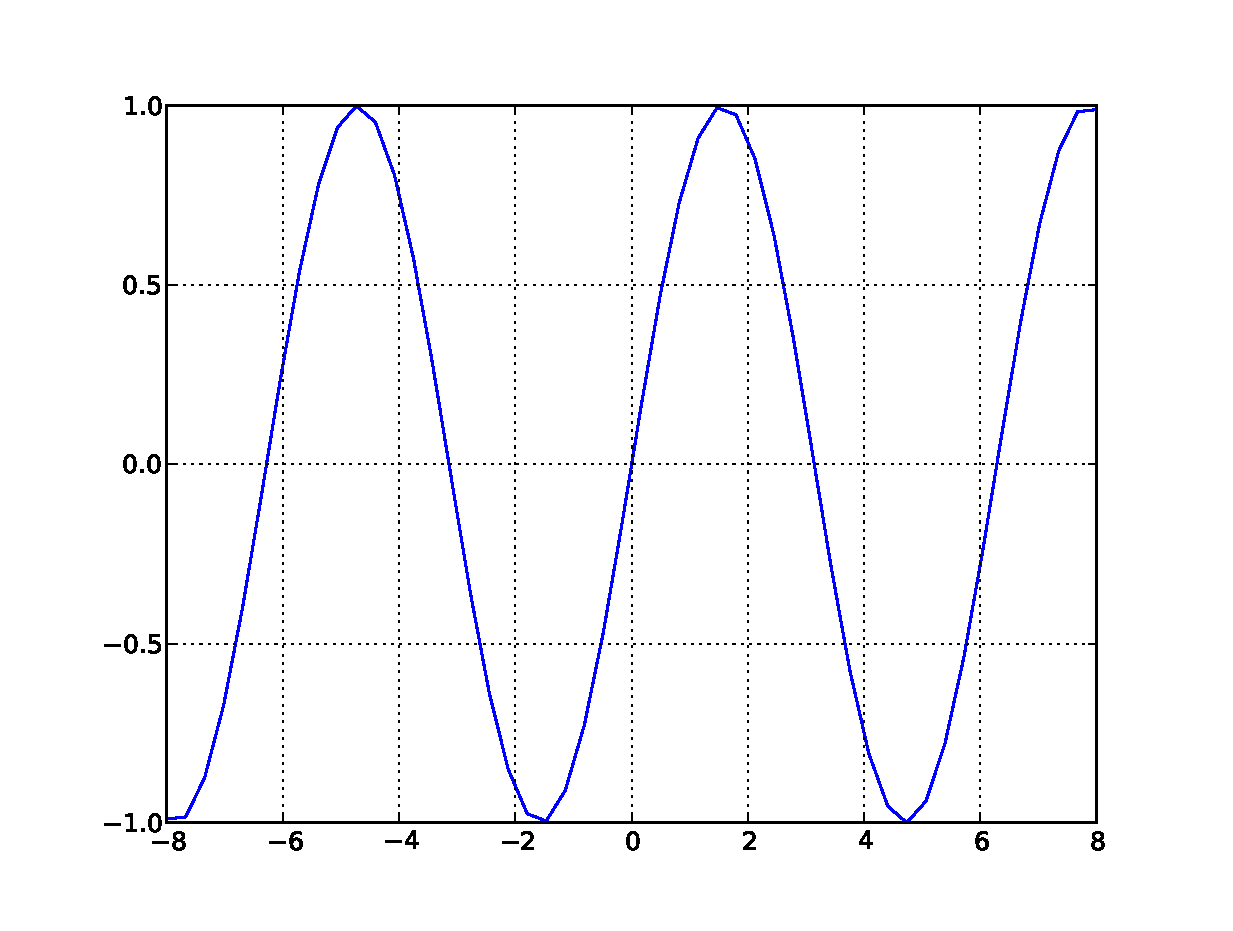
\includegraphics[scale=0.4]{raices00.eps} 
% \end{figure}
% \end{frame}
% \begin{frame}
% Las raíces de un polinomio pueden ser reales o complejas.
% \\
% \bigskip
% Si un polinomio tiene coeficientes reales
% \[ a_{0},a_{1},a_{2},\ldots,a_{n-1},a_{n} \]
% entonces todas las raíces complejas siempre ocurrirán en pares conjugados complejos.
% \end{frame}
% \begin{frame}
% Por ejemplo, un polinomio cúbico tiene la siguiente
% forma general:
% \[ f(x)= a_{0}x^{3}+a_{1}x^{2}+a_{2}x+a_{3}\]
% \setbeamercolor{item projected}{bg=red!70!black,fg=white}
% \setbeamertemplate{enumerate items}[circle]
% \begin{enumerate}
% \item Tres raíces reales distintas.
% \item Una raíz real con multiplicidad 3.
% \item Una raíz real simple y una raíz real con multiplicidad 2.
% \item Una raíz real y un par conjugado complejo.
% \end{enumerate}
% \end{frame}
% \begin{frame}[fragile]
% \frametitle{Tres raíces distintas}
% \begin{minipage}{5cm}
% \fontsize{12}{12}\selectfont
% \[ \begin{split}
% f(x)=& x^{3} - 3x^{2}-x+3 \\
% =& (x-3)(x+1)(x-1)
% \end{split} \]
% Las raíces son:
% \[ \begin{split}
% x_{1} =& 3 \\
% x_{2} =& -1 \\
% x_{3} =& 1 \\
% \end{split}\]
% \end{minipage}
% \hspace{0.5cm}
% \begin{minipage}{4.5cm}
% \begin{figure}
% 	\centering
% 	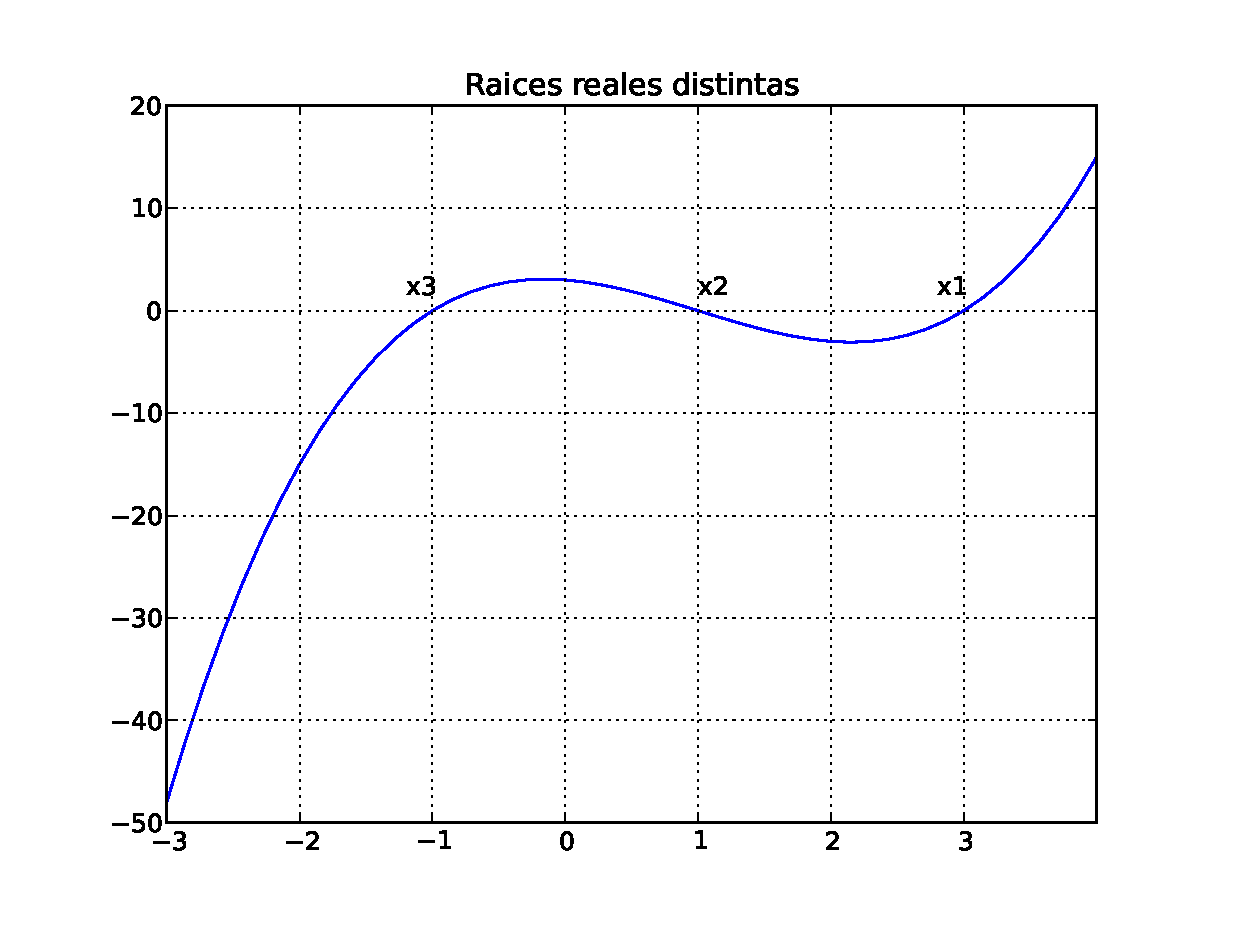
\includegraphics[scale=0.3]{raices01.eps} 
% \end{figure}
% \end{minipage}
% \end{frame}
% \begin{frame}[fragile]
% \frametitle{Raíz real con multiplicidad 3}
% \begin{minipage}{5cm}
% \fontsize{12}{12}\selectfont
% \[ \begin{split}
% f(x)=& x^{3} - 6x^{2} + 12x - 8 \\
% =& (x-2)^{3}
% \end{split} \]
% Las raíces son:
% \[ \begin{split}
% x_{1} =& 2 \\
% x_{2} =& 2 \\
% x_{3} =& 2 \\
% \end{split}\]
% \end{minipage}
% \hspace{0.5cm}
% \begin{minipage}{4.5cm}
% \begin{figure}
% 	\centering
% 	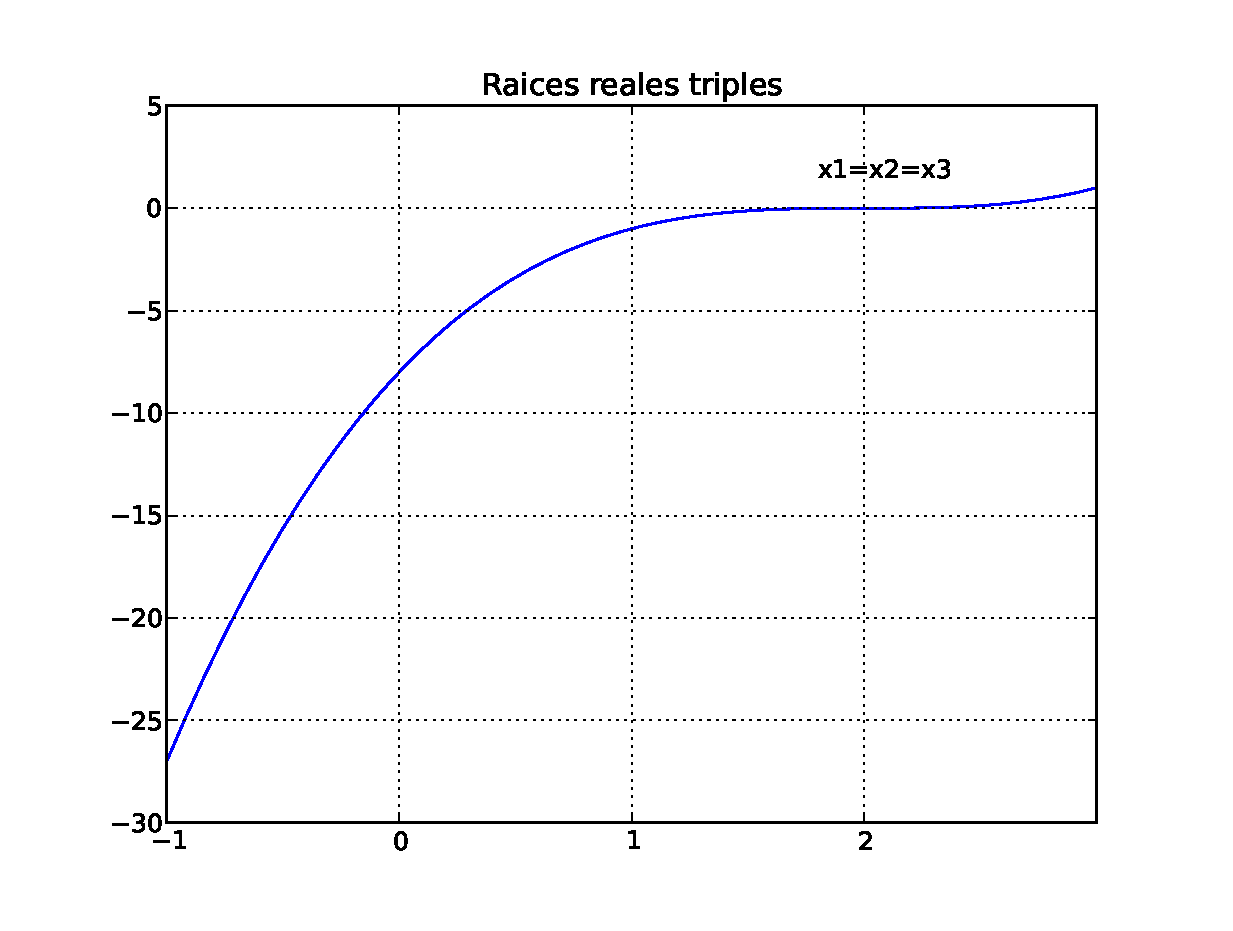
\includegraphics[scale=0.3]{raices02.eps} 
% \end{figure}
% \end{minipage}
% \end{frame}
% \begin{frame}[fragile]
% \frametitle{Raíz real simple y \\ una raíz real con multiplicidad 2}
% \begin{minipage}{5cm}
% \fontsize{12}{12}\selectfont
% \[ \begin{split}
% f(x)=& x^{3} - 12x + 16 \\
% =& (x+4)(x-2)^{2}
% \end{split} \]
% Las raíces son:
% \[ \begin{split}
% x_{1} =& -4 \\
% x_{2} =& 2 \\
% x_{3} =& 2 \\
% \end{split}\]
% \end{minipage}
% \hspace{0.5cm}
% \begin{minipage}{4.5cm}
% \begin{figure}
% 	\centering
% 	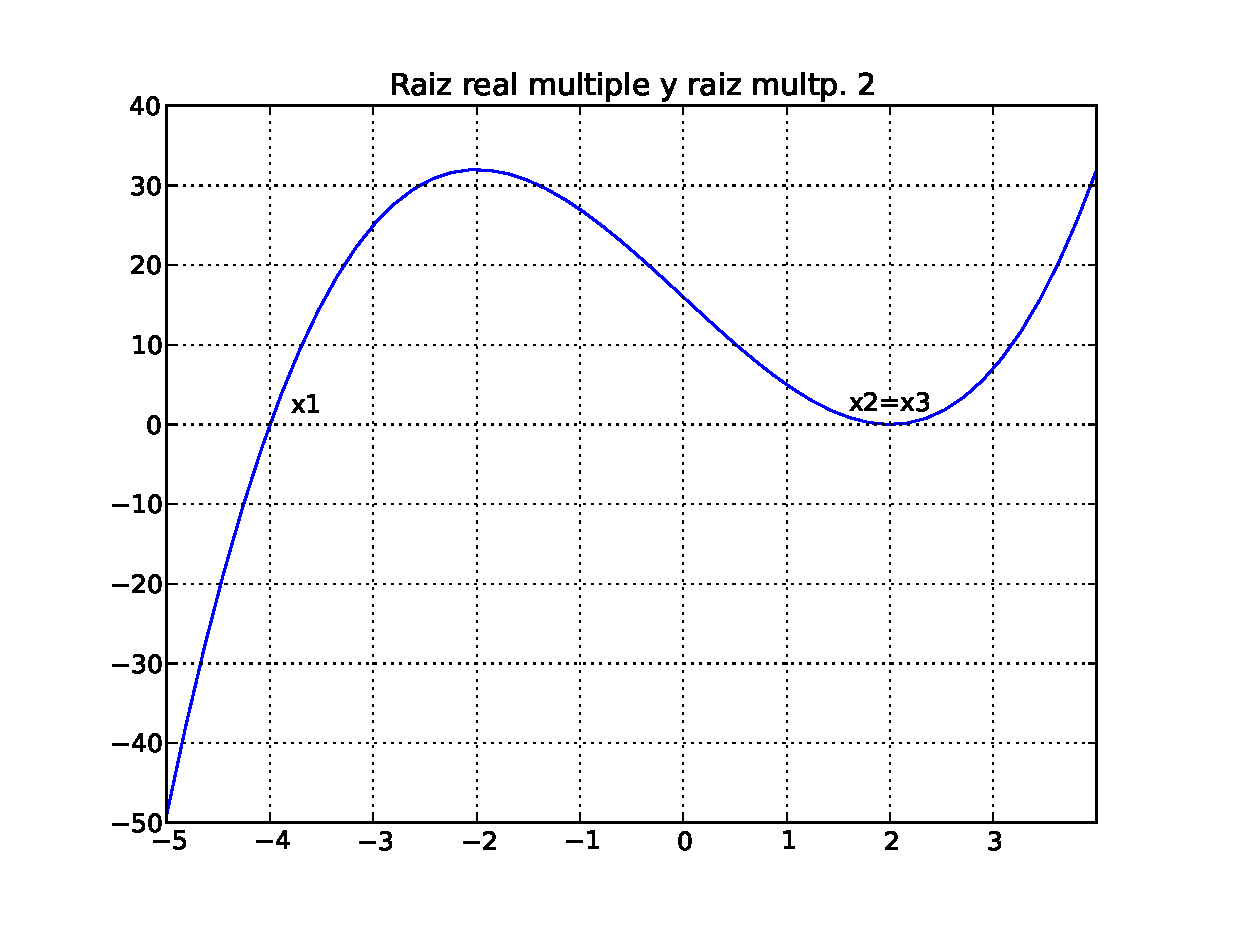
\includegraphics[scale=0.3]{raices03.eps} 
% \end{figure}
% \end{minipage}
% \end{frame}
% \begin{frame}[fragile]
% \frametitle{Raíz real y un par conjugado complejo}
% \begin{minipage}{5cm}
% \fontsize{12}{12}\selectfont
% \[ \begin{split}
% f(x)=& x^{3} - 2x^{2}- 3x +10  \\
% =& (x+2)(x- (2+i))* {}\\
% *& (x-(2-i))
% \end{split} \]
% Las raíces son:
% \[ \begin{split}
% x_{1} =& -2 \\
% x_{2} =& 2+i \\
% x_{3} =& 2-i \\
% \end{split}\]
% \end{minipage}
% \hspace{0.5cm}
% \begin{minipage}{4.5cm}
% \begin{figure}
% 	\centering
% 	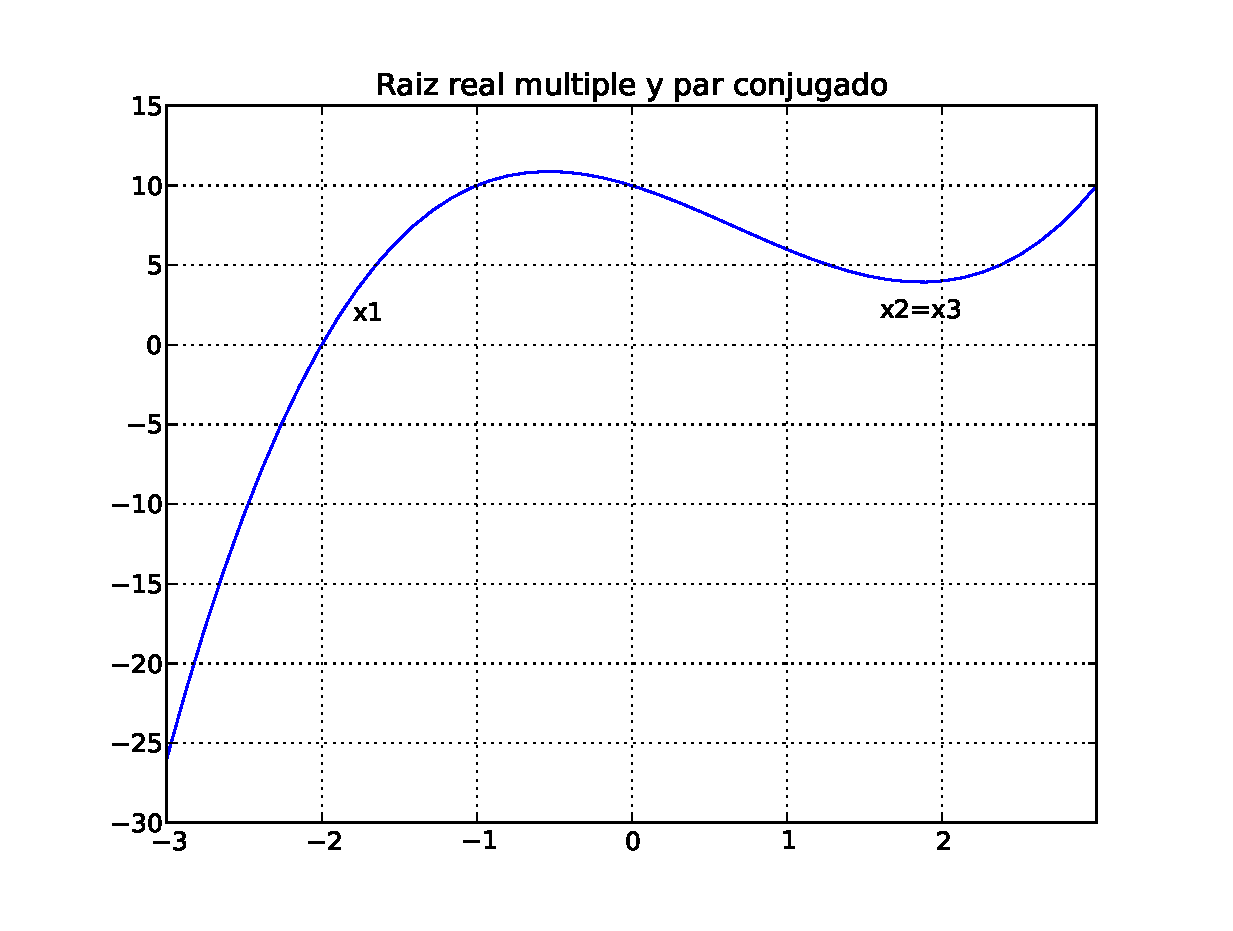
\includegraphics[scale=0.3]{raices04.eps} 
% \end{figure}
% \end{minipage}
% \end{frame}
% \section{Funciones algebraicas}
% \begin{frame}
% \frametitle{Funciones algebraicas}
% Sea $g=f(x)$ la función expresada como
% \[ f_{n}y^{n} + f_{n-1}y^{n-1} + \ldots + f_{1}y + f_{0} = 0 \]
% Donde $f_{i}$ es un polinomio de orden $i$ en $x$.
% \\
% \bigskip
% Los polinomios son un caso simple de funciones algebraicas que se representan generalmente como
% \[f_{n}(x) = a_{0} + a_{1}x + a_{2} x^{2}+ \ldots +a_{n}x^{n} \]
% Donde $n$ es el orden del polinomio.
% \end{frame}
% \section{Funciones trascendentales}
% \begin{frame}
% \frametitle{Funciones trascedentales}
% Son aquellas que no son algebraicas.
% \\
% \bigskip
% Comprenden a las funciones trigonométricas, exponenciales, logarítmicas, entre otras.
% \\
% \bigskip
% Ejemplos:
% \begin{itemize}
% \item \[ f(x)=ln(x^{2}-1) \]
% \item \[g(x)=e^{-0.2x} \sin(3x-5) \]
% \end{itemize}
% \end{frame}
% \begin{frame}
% Los métodos numéricos estándar para encontrar
% raíces pueden clasificarse en dos rubros:
% \\
% \bigskip
% \textbf{1.} La determinación de las raíces reales de ecuaciones algebraicas y trascendentales. Las técnicas a emplear en estos casos se diseñaron con el fin de encontrar el valor de una raíz simple de acuerdo con un conocimiento previo de su posición aproximada.
% \end{frame}
% \begin{frame}
% \textbf{2.} La determinación de todas las raíces reales y complejas de un polinomio, para lo cual los métodos numéricos estén diseñados específicamente para polinomios. 
% \\
% \bigskip
% Determinan sistemáticamente todas las raíces del polinomio en lugar de hacerlo sólo con una, dada la posición aproximada.
% \end{frame}
% \section{Método de incrementos sucesivos}
% \begin{frame}
% \frametitle{Método de incrementos sucesivos}
% Podemos aproximar mucho mejor las raíces de una función, cuando la graficamos.
% \\
% \bigskip
% Con una gráfica general de unos cuantos puntos, tendríamos lo necesario para considerar los valores de las raíces.
% \\
% \bigskip
% El método de búsqueda incremental es una herramienta útil que podemos adoptar en conjunto con otras estrategias de cálculo de raíces, por sí sólo, éste método no nos ofrece más que una referencia sobre en dónde podrían estar esas raíces.
% \end{frame}
% \begin{frame}
% La idea básica detrás del método de búsqueda incremental es simple: si $f(x_{1})$ y $f(x_{2})$ tienen signos opuestos, entonces hay al menos una raíz en el intervalo $(x_{1}, x_{2})$.
% \end{frame}
% \begin{frame}[fragile]
% \frametitle{Caso en donde es posible encontrar la raíz}
% \begin{center}
% 	\begin{tikzpicture}[font=\footnotesize, scale=1.3]
% 		\draw[<->](0,0) -- (6,0);
% 		\draw[<->](3,-2) -- (3,2);
% 		\draw [red] (0.5,1.5) .. controls (2,0.2) and (4,-1) .. (5.5,-1.5);
% 		\draw[dashed] (1,0) -- (1,1.1);
% 		\draw (0.9,-0.2) node {a}; 
% 		\draw (1.2,1.4) node {f(a)};
% 		\draw[dashed] (5,0) -- (5,-1.33);
% 		\draw (5,0.2) node {b}; 
% 		\draw (5,-1.7) node {f(b)};
% 		\draw(4.5,1.5) node {$f(a)*f(b)<0$};
% 	\end{tikzpicture}
% \end{center}
% \end{frame}
% \begin{frame}
% \frametitle{Caso en donde no es posible encontrar la raíz}
% \begin{center}
% 	\begin{tikzpicture}[font=\footnotesize, scale=1.3]
% 		\draw[<->](0,0) -- (6,0);
% 		\draw[<->](3,-1) -- (3,3);
% 		\draw [red] (0.5,2.5) .. controls (2.5,0.5) and (3.5,0.5) .. (5.5,2.5);
% 		\draw [dashed] (1,0) -- (1,2.1);
% 		\draw (1,-0.2) node {a};
% 		\draw (1.1,2.2) node {f(a)};
% 		\draw [dashed] (4.5,0) -- (4.5,1.65);
% 		\draw (4.5,-0.2) node {b};
% 		\draw (4.5, 2) node {f(b)};
% 		\draw (5,3.5) node {$f(a)*f(b)>0$};
% 	\end{tikzpicture}
% \end{center}
% \end{frame}
% \begin{frame}
% Si el intervalo es lo suficientemente pequeño, es probable que contenga una sola raíz. Así, los ceros de $f(x)$ puede ser detectados mediante la evaluación de la función a intervalos $\Delta x$ y mirando cuando se presente un cambio de signo en la función.
% \end{frame}
% \begin{frame}
% Hay varios problemas con el método de búsqueda incremental:
% \setbeamercolor{item projected}{bg=red!70!black,fg=white}
% \setbeamertemplate{enumerate items}[circle]
% \begin{enumerate}[<+->]
% \item Es posible perder dos raíces muy próximas entre sí, si el incremento de búsqueda $\Delta x$ es mayor que la separación de las raíces.
% \item Una raíz doble (dos raíces que coinciden) no será detectada.
% \item Algunas singularidades de $f(x)$ se puede confundir con raíces. Por ejemplo, $f(x) = \tan x$. Tiene cambios de signo en $x = \pm 1/2 n\pi$ con $n = 1, 3, 5,\ldots$
% \end{enumerate}
% \end{frame}
% \begin{frame}
% Estos puntos no son ceros verdaderos, ya que la función no cruza el eje $x$.
% \begin{figure}
% 	\centering
% 	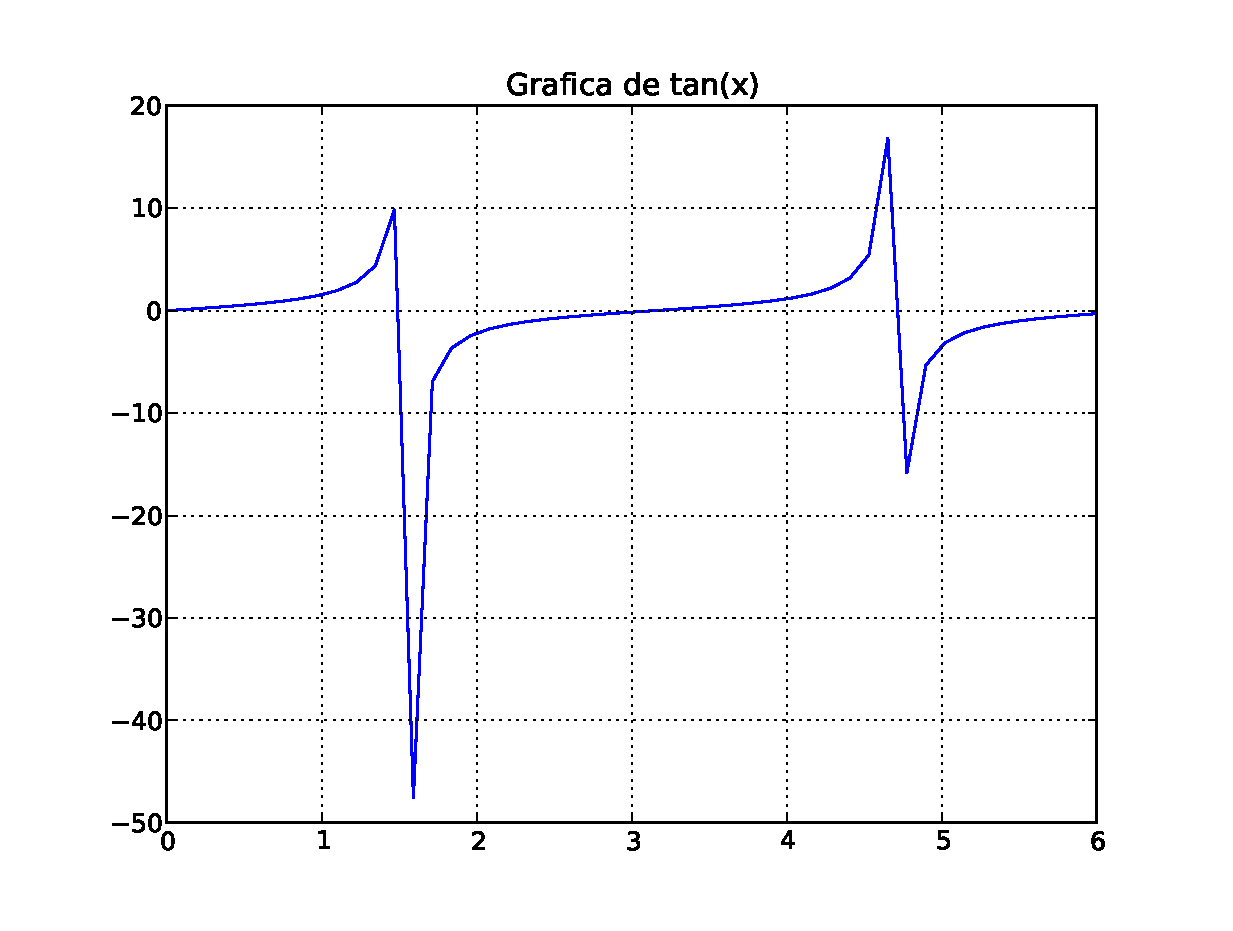
\includegraphics[scale=0.4]{raices05.eps} 
% \end{figure}
% \end{frame}
% \subsection{Código Método de incrementos sucesivos}
% \begin{frame}
% \frametitle{Código Método de incrementos sucesivos}
% El código busca un cero de la función $f$ que proporciona el usuario en el intervalo
% $(a,b)$ en incrementos de $dx$.
% \\
% \bigskip
% Se devuelve el intervalo $(x_{1}, x_{2})$ donde se encuentra la raíz, si la búsqueda
% se ha realizado correctamente; se devuelve $x_{1} = x_{2} = \mathsf{None}$ cuando no se encontraron raíces.
% \\
% \bigskip
% Luego de que se encontró la primera raíz, (la más cercana al punto $a$), se puede llamar de nuevo al procedimiento, sustitiyendo $x_{2}$ con el fin de encontrar la siguiente raíz. Esto se puede repetir siempre y cuando se detecta una raíz.
% \end{frame}
% \begin{frame}[fragile]
% \begin{lstlisting}[basicstyle=\ttfamily\normalsize, columns=fullflexible]
% def buscaraiz(f,a,b,dx):
%     x1 = a; f1 = f(a)
%     x2 = a + dx; f2 = f(x2)
%     while f1*f2 > 0.0:
%         if x1 >= b: return None
%         x1 = x2; f1 = f2
%         x2 = x1 + dx; f2 = f(x2)
%     else:
%         return x1,x2
% \end{lstlisting}
% \end{frame}
% \begin{frame}
% \frametitle{Ejemplo}
% Usa el método de incrementos sucesivos y con $\Delta x= 0.2$, para estimar la raíz con el valor positivo más pequeño de la función:
% \[ f(x) = x^{3} - 10 x^{2} + 5\]
% \end{frame}
% \begin{frame}
% \frametitle{Revisión general de la función}
% Conviene graficar inicialmente la función para tener una idea sobre los intervalos iniciales, \emph{evita proponer valores del intervalo muy cercanos a la raíz}, lo que se busca es que revises la implementación del código.
% \begin{figure}
% 	\centering
% 	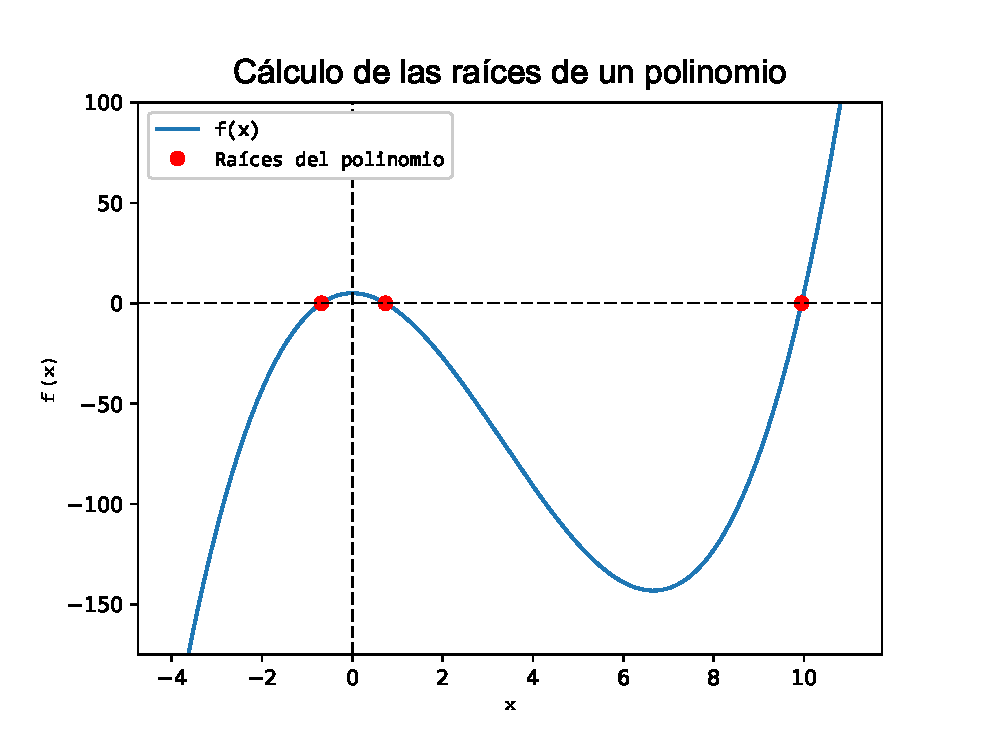
\includegraphics[scale=0.4]{Imagenes/funcion_raiz_01.eps} 
% \end{figure}
% \end{frame}
% \begin{frame}
% \frametitle{Consideraciones importantes.}
% Si al momento de graficar la función para explorar un poco, notamos que de izquierda a derecha tenemos las tres raíces $x_{0}, x_{1}, x_{2}$, aunque aún no sabemos su valor, podemos estimar en qué intervalo se encuentran.
% \\
% \bigskip
% El algoritmo de incrementos sucesivos debería de informarnos en qué intervalos se encuentran las raíces.
% \end{frame}
% \begin{frame}
% \frametitle{Raíces del polinomio}
% El problema pide calcular la raíz positiva más pequeña del polinomio de tercer grado, de acuerdo a la gráfica, la raíz buscada es $x_{1}$, ya que $x_{0}<0$ y $x_{2} > x_{1}$.
% \begin{figure}
% 	\centering
% 	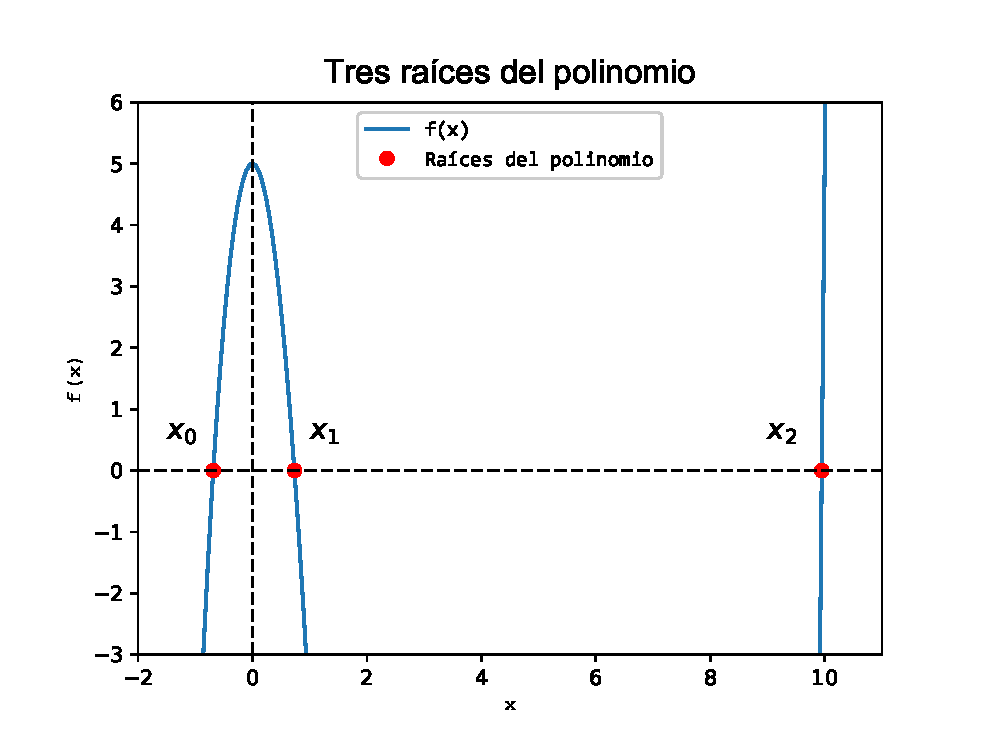
\includegraphics[scale=0.5]{funcion_raiz_02.eps} 
% \end{figure}
% \end{frame}
% \begin{frame}
% \frametitle{Intervalo de inicio}
% Con toda tranquilidad presentamos el intervalo de inicio para el método de incrementos sucesivos para determinar el intervalo en donde se encuentra $x_{1}$: la raíz positiva más pequeña de $f(x)$.
% \begin{figure}
% 	\centering
% 	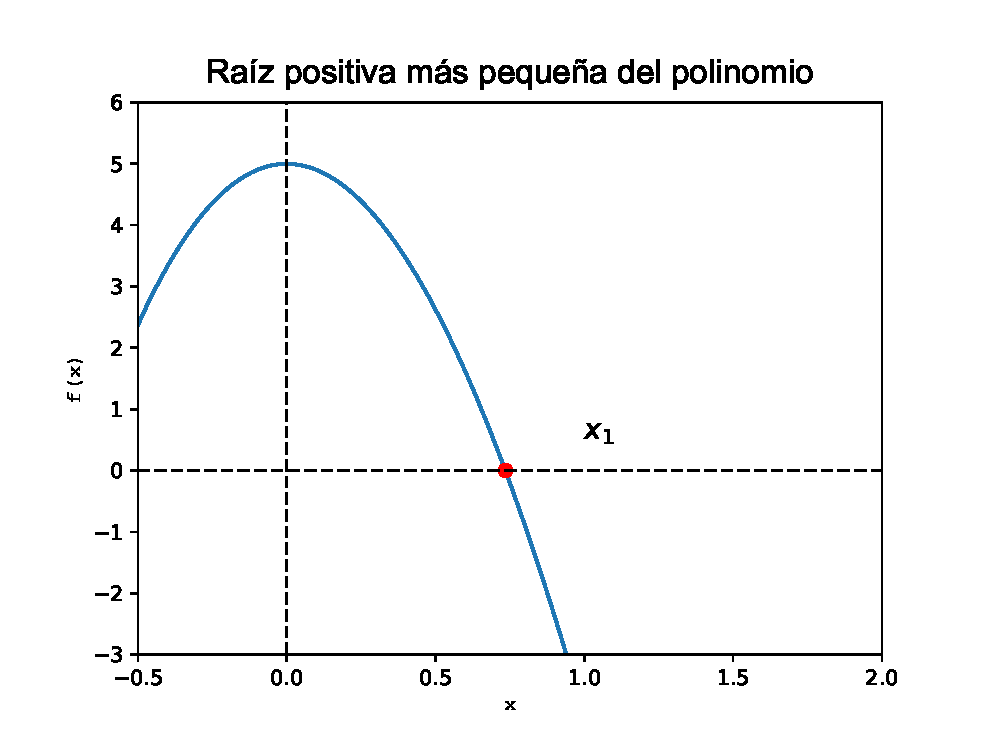
\includegraphics[scale=0.5]{funcion_raiz_03.eps} 
% \end{figure}
% \end{frame}

% \begin{frame}[fragile]
% \begin{lstlisting}[basicstyle=\ttfamily\normalsize, columns=fullflexible]
% def f(x): return x**3 - 10*x**2 + 5.

% a, b, dx = (0.0,1.5, 0.2)

% print ('El intervalo es: ')
% x1, x2 = buscaraiz(f,a,b,dx)
% print (x1,x2)
% \end{lstlisting}
% \end{frame}
% \begin{frame}
% El código incluye el intervalo $[0.0, 1,5]$, pero una vez que localiza que ya no hay cambio de signo, se detiene.
% \\
% \bigskip
% ¿Cómo podríamos mejorar nuestro código para que sin importar el valor inicial del intervalo, realice un ``escaneo'' sobre todo el eje de las abscisas? De tal manera que nos reporte el total de raíces que existen y en los intervalos en dónde se encuentran. (Tomando en cuenta que usaríamos un intervalo inicial razonable)
% \end{frame}
\end{document}